\documentclass[12pt, parskip, DIV=14]{scrbook}

\usepackage{a4wide,times}
% \usepackage{fontspec}
\usepackage{tikz}
\usepackage[type1]{quattrocento}
% \usepackage{amssymb}
\usepackage[notext,lcgreekalpha]{stix}
\usepackage{amsmath}
\usepackage{amsfonts}
\usepackage{amsthm}
\usepackage{mathtools}
\usepackage{stmaryrd}
\usepackage{hyperref}
\usepackage[nameinlink]{cleveref}
\usepackage{multirow}
\usepackage{relsize}

\usepackage{newunicodechar}

\usepackage[textsize=tiny]{todonotes}
\usepackage{xargs}
\newcommandx{\info}[2][1=]{\todo[linecolor=blue,backgroundcolor=blue!25,bordercolor=blue,#1]{#2}}

\usepackage[zerostyle=d]{newtxtt}
\usepackage[T1]{fontenc}

\setkomafont{disposition}{\scshape\bfseries}

\usepackage[numbers]{natbib}
\bibliographystyle{plainnat}

% Don't include subsections in ToC
\setcounter{tocdepth}{1}

\DeclareMathAlphabet{\mathpzc}{OT1}{pzc}{m}{it}
\DeclareMathOperator\prof{\nvrightarrow}
\DeclareMathOperator\ltri{\langle\mkern-3mu[}
\DeclareMathOperator\rtri{]\mkern-3mu\rangle}
\DeclareMathOperator\lapp{+\mkern-3mu+}
\newcommand{\defeq}{\vcentcolon\equiv}
\renewcommand{\circ}{\vysmwhtcircle}
\mathchardef\mhyphen="092C
\newcommand{\Nat}{\operatorname{Nat}}
\newcommand{\SM}{\operatorname{SM}}
\newcommand{\Fin}{\operatorname{Fin}}
\newcommand{\ap}{\operatorname{ap}}
\newcommand{\idp}{\operatorname{idp}}
\newcommand{\coe}{\operatorname{coe}}
\newcommand{\transport}{\operatorname{transport}}
\newcommand{\iscontr}{\operatorname{is\mhyphen contr}}
\newcommand{\isprop}{\operatorname{is\mhyphen prop}}
\newcommand{\hasallpaths}{\operatorname{has\mhyphen all\mhyphen paths}}
\newcommand{\isset}{\operatorname{is\mhyphen set}}
\newcommand{\isgpd}{\operatorname{is\mhyphen gpd}}
\newcommand{\haslevel}{\operatorname{has\mhyphen level}}
\newcommand{\Suc}{\operatorname{S}}
\newcommand{\hProp}{\mathbf{hProp}}
\newcommand{\hSet}{\mathbf{hSet}}
\newcommand{\hGpd}{\mathbf{hGpd}}
\DeclareMathOperator\daytensor{\widehat\otimes}
\newcommand{\dayid}{\operatorname{\hat{I}}}
\newcommand{\Lan}{\operatorname{Lan}}
\newcommand{\List}{\operatorname{List}}
\newcommand{\Gpd}{\mathbf{Gpd}}
\newcommand{\Quot}{\operatorname{Quot}_C(R)}
\newcommand{\q}{\operatorname{q}}
\newcommand{\rel}{\operatorname{rel}}
\newcommand{\relidp}{\operatorname{rel\mhyphen idp}}
\newcommand{\reldot}{\operatorname{rel\mhyphen \cdot}}
\newcommand{\qs}{\operatorname{q}^*}
\newcommand{\rels}{\operatorname{rel}^*}
\newcommand{\relidps}{\operatorname{rel\mhyphen idp}^*}
\newcommand{\reldots}{\operatorname{rel\mhyphen \cdot}^*}
\newcommand{\SetQuot}{\operatorname{SetQuot}_C(R)}
\newcommand{\GpdQuot}{\operatorname{GpdQuot}_C(R)}
\newcommand{\Rrefl}{\operatorname{R\mhyphen is\mhyphen refl}}
\newcommand{\Rsym}{\operatorname{R\mhyphen is\mhyphen sym}}
\newcommand{\Rtrans}{\operatorname{R\mhyphen is\mhyphen trans}}
\newcommand{\here}{\operatorname{here}}
\newcommand{\there}{\operatorname{there}}
\newcommand{\firsthere}{\operatorname{first\mhyphen here}}
\newcommand{\remfirsthere}{\operatorname{remove\mhyphen first\mhyphen here}}
\newcommand{\monfold}{\operatorname{monoid\mhyphen fold}}
\newcommand{\monfoldconst}{\operatorname{monoid\mhyphen fold\mhyphen is\mhyphen const}}
\newcommand{\monfoldinv}{\operatorname{monoid\mhyphen fold}'\mkern-3mu\operatorname{\mhyphen is\mhyphen perm\mhyphen invariant}}
\newcommand{\trans}{\operatorname{trans\mhyphen perm}}
\newcommand{\ListPerm}{\operatorname{ListPerm}}
\newcommand{\remove}{\operatorname{remove}}
\newcommand{\lpnil}{\operatorname{lpnil}}
\newcommand{\lpcons}{\operatorname{lpcons}}
\newcommand{\nil}{\operatorname{nil}}
\newcommand{\iswconst}{\operatorname{is\mhyphen wconst}}
\newcommand{\iscoh}{\operatorname{is\mhyphen coh}}
\newcommand{\inl}{\operatorname{inl}}
\newcommand{\inr}{\operatorname{inr}}
\newcommand{\fresh}{\operatorname{fresh}}
\newcommand{\inc}{\operatorname{inc}}
\newcommand{\botrec}{\operatorname{\bot\mhyphen rec}}
\newcommand{\finempty}{\operatorname{Fin0\mhyphen\bot}}
\newcommand{\finunit}{\operatorname{Fin1\mhyphen\top}}
\newcommand{\smfin}{\operatorname{SM\mhyphen Fin}}
\newcommand{\Esp}{\mathbf{Esp}}
\newcommand{\op}[1]{#1^\mathrm{op}}
\newcommand{\id}{\operatorname{id}}
\newcommand{\spec}[2]{#1 \rightwavearrow #2}

\newunicodechar{Σ}{$\Sigma$}
\newunicodechar{⊗}{$\otimes$}
\newunicodechar{ø}{$\daytensor$}
\newunicodechar{ı}{$\widehat\text{I}$}
\newunicodechar{×}{$\times$}
\newunicodechar{→}{$\to$}
\newunicodechar{λ}{$\mathbf{\lambda}$}
\newunicodechar{₀}{$_\text{0}$}
\newunicodechar{₁}{$_\text{1}$}
\newunicodechar{₂}{$_\text{2}$}
\newunicodechar{∎}{$\smblksquare$}
\newunicodechar{≃}{$\simeq$}
\newunicodechar{⟨}{$\langle$}
\newunicodechar{⟩}{$\rangle$}
\newunicodechar{∀}{$\forall$}
\newunicodechar{⁻}{$^-$}
\newunicodechar{¹}{$^\text{1}$}
\newunicodechar{∘}{$\circ$}
\newunicodechar{∈}{$\in$}
\newunicodechar{∪}{$\cup$}
\newunicodechar{↓}{$\downarrow$}

%%% Hack for wide hats %%%
\usepackage{scalerel,stackengine}
\stackMath
\newcommand\reallywidehat[1]{%
\savestack{\tmpbox}{\stretchto{%
  \scaleto{%
    \scalerel*[\widthof{\ensuremath{#1}}]{\kern-.6pt\bigwedge\kern-.6pt}%
    {\rule[-\textheight/2]{1ex}{\textheight}}%WIDTH-LIMITED BIG WEDGE
  }{\textheight}%
}{0.5ex}}%
\stackon[1pt]{#1}{\tmpbox}%
}
\parskip 1ex

% TeXCount Parsing Rules

%TC:envir tabular [] text

\title{Generalised Species of Structures in Homotopy Type Theory Using Agda}
\author{Rupert Horlick (rh572) \\
  \large Homerton College }
\date{}
\subject{Part III Dissertation}
\publishers{Supervisor: Prof. M. Fiore \\
  \vspace{3em}
  \centering\large
  University of Cambridge \\
  Computer Laboratory \\
  William Gates Building \\
  15 JJ Thompson Avenue \\
  Cambridge, CB3 0FD \\
  United Kingdom}

\begin{document}

\frontmatter

\maketitle

\addchap*{Abstract}

\textbf{Generalised Species of Structures in Homotopy Type Theory Using Agda}

There is an increasing interest in computer-assisted formalisation in Computer Science and Mathematics. The aim of this dissertation was to explore the use of some of the most cutting-edge tools and libraries in formalising the theory of generalised species of structures \citep{fiore2008cartesian}. Species of structures provide a framework for reasoning about data structures of all kinds, for example allowing us to prove that two structures are interchangeable. This could allow compiler optimisations that automatically choose the most efficient data structure for a particular application while preserving semantics. This theory includes a calculus of operations such as addition and even differentiation of structures. The formalisation embeds category-theoretic notions in the constructs of homotopy type theory, a novel approach to the formalisation of category theory.

\newpage

Word count: 10,183 (calculated using TeXcount)

\tableofcontents

\mainmatter

\chapter{Introduction}
\label{chap:intro}

There is an increasing interest in computer-assisted formalisation in Computer Science and Mathematics. From the lowest level hardware verification to the most abstract pure mathematics, computers have a role to play in making our lives easier. They can solve increasingly complex systems of constraints, hold vast pools of knowledge, and provide important modular organisation of proofs, leaving the most interesting and creative problems to the humans. This excitement is showcased by events such as Big Proof, to be held at the Isaac Newton Institute this summer.

The aim of this dissertation was to explore the use of some of the most cutting-edge tools and libraries in formalising the theory of generalised species of structures \citep{fiore2008cartesian}. This theory aims to provide a category-theoretic calculus for bijective proofs of combinatorial identities, so it makes sense to do so constructively. Thus, Agda \citep{norell2007towards}, an implementation of Martin-L\"of type theory \citep{martin1975intuitionistic}, seemed like the tool of choice.

We further wanted to explore this formalisation in the context of homotopy type theory \citep{hottbook}, an interpretation of Martin-L\"of type theory based on homotopy theory. A major goal of the homotopy type theory project is to provide a common foundation for mathematicians working in formalisation, so this project provides another test of its worth. The HoTT-Agda library \citep{hottagda} is a thorough, well-structured implementation of homotopy type theory that played a role in our decision to use Agda.

There were two choices of how to formalise the theory. The first option was to develop category theory from scratch using some of the foundations outlined in \citep{hottbook}. The second option was to interpret the constructs of homotopy type theory as categorical structures, developing the theory internally to the type theory. This is a novel approach and the one we chose to follow.

The project has three main parts. First the formalisation of presheaves, a type of categorical functor, along with operations for manipulating them. Second the formalisation of the free strict symmetric-monoidal completion that generalises the set-theoretic finite-multiset construction. This construction was the most significant challenge of the project and we ended up having two implementations of it. Lastly, with the first two parts, the formalisation of generalised species themselves. This includes the differential calculus of species, a set of operations and laws for combination and manipulation of species. This culminates in the species version of the Leibniz rule for differentiation.

\section{Related Work}

The study of species began with the work of \citet{joyal1981une, joyal1986foncteurs} who gave the original definition and showed their relation to exponential power series. This work was explored further by \citet{bergeron1998combinatorial} in an extensive volume. The notion of species was expanded to that of generalised species of structures by \citet{fiore2008cartesian} who showed the Cartesian Closure of the bicategory of generalised species and showed the links between species and models of linear logic. Further \citet{fiore2005mathematical} defined the differential calculus of species.

Homotopy type theory began in 2012-13 during a Special Year on Univalent Foundations of Mathematics at the Institute of Advanced Study. The Special Year led to the official book \citep{hottbook}, a thorough look at homotopy type theory and its current applications. The PhD thesis of \citet{yorgey2014combinatorial} defines Joyal's species in the context of homotopy type theory, but was not formalised.

The formalisation of a theory of groupoids in homotopy type theory requires higher structure. The work of \citet{hou2017higher} looks specifically at the formalisation of such structures in Agda. The work of \citet{kraus2014general} generalises some useful notions from the former that apply when defining actions on groupoids.

\chapter{Background}

\section{Category Theory}
\label{sec:cattheory}

We assume that the reader has a grasp of the basic notions of category theory. That is we assume familiarity with categories, functors, natural transformations, initial/terminal objects, products/coproducts, limits/colimits in general, exponentials, Cartesian Closed Categories, and the Yoneda Lemma.

Two notions that do not usually appear in introductory courses are groupoids and ends/coends. These will both be required throughout this dissertation, so their definitions will be discussed here.

\paragraph{Groupoids}

A groupoid is a special kind of category, specifically one where every morphism has an inverse. This property induces an isomorphism between $\mathbb{G}$ and $\mathbb{G}^\mathrm{op}$ for every groupoid $\mathbb{G}$.

\paragraph{Ends/Coends}

Ends/coends are a type of limit/colimit over functors of the form $F : \mathbb{C}^\mathrm{op} \times \mathbb{C} \to \mathbb{D}$. For such a functor, a wedge $w : e \to F$ is an object $w : \mathbb{D}$ and a family of morphisms $e_c : w \to F(c,c)$, for each $c \in \mathbb{C}$, such that, for every morphism $f : c \to c'$ in $\mathbb{C}$, the diagram
\begin{center}
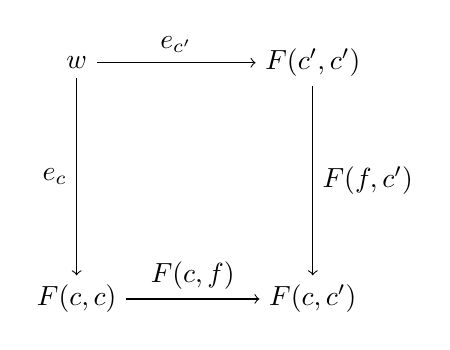
\begin{tikzpicture}[node distance=3cm and 1cm]
  \node (Px)               {$w$};
  \node (Qx) [right of=Px] {$F(c' , c')$}
    edge [<-] node[above] {$e_{c'}$} (Px);
  \node (Py) [below of=Px] {$F(c , c)$}
    edge [<-] node [left] {$e_c$} (Px);
  \node      [below of=Qx] {$F(c , c')$}
    edge [<-] node [above] {$F(c , f)$} (Py)
    edge [<-] node [right] {$F(f , c')$} (Qx);
\end{tikzpicture}
\end{center}
commutes. We can compose with a map $g : v \to w$ to form a new wedge $e~f : v \to F$. An end is a universal wedge, i.e. a wedge $e : w \to F$ such that for any other wedge $e' : w' \to F$, the latter factors through the former by a unique map $w' \to w$. The dual notion of cowedge leads to the definition of coends.

%What is the intuition for this?

\section{Homotopy Type Theory}
\label{sec:HoTT}

Homotopy type theory is a new area of mathematics that combines homotopy theory and Martin-L\"of type theory \citep{martin1975intuitionistic}. Homotopy theory deals with \textit{spaces} and \textit{continuous maps} between spaces, up to homotopy. A \textit{homotopy} between two continuous maps is a ``continuous'' deformation of one map into the other. Two spaces $X$ and $Y$ are \textit{homotopy equivalent}, $X \simeq Y$, if we have continuous maps in both directions, whose compositions both have homotopies to the identity maps.

Homotopy type theory uses these spaces as the interpretation of type theory. The statement ``$a$ has type $A$'' or $a : A$, is taken to mean ``$a$ is a point in the space $A$''. Type constructions, such as functions and product, can be seen as homotopy-invariant constructions on spaces. All types themselves have types, which are called universes, and are denoted $U$. Type universes are complicated and not well understood, but we will explore their analogy to the category theoretic $\mathbf{Set}$ in \Cref{chap:interp}.

\paragraph{A Quick Note on Equality} To talk about homotopy type theory we need several notions of equality. \textit{Definitional equality}, denoted $\defeq$, allows us to make two terms equal by definition. \textit{Judgemental equality}, denoted $\equiv$, means that two terms compute to the same normal form based on existing definitions. Finally \textit{propositional equality}, denoted $=$, is internal to type theory and will be defined below.

\paragraph{Type Formers}

To make type theory useful we need the ability to build new types. Defining a type means specifying how to form values of the type, how to eliminate values of the type, and how to compute with values of the type. These specifications are called introduction rules, elimination rules, and computation rules.

Many common types fall under the label of \textit{inductively defined} types. These consist of a number of constructors with optional arguments; an application of each constructor is an introduction rule. The elimination and computation rules can also be derived from the constructors. To eliminate a value of an inductively defined type, one must perform case analysis on the value and provide a result for each case. Given a specific value of the type, computation picks the correct result based on the case analysis.

Some types are not defined inductively. These types do not use the framework of constructors given above, and have to define their own introduction, elimination, and computation rules. Important examples of this are the basic function and product types, as well as their dependent versions, $\Pi$ and $\Sigma$ types.

Functions are formed using $\lambda$-abstraction and eliminated using function application. The computation rule says $$(\lambda x . C(x))(a) \mapsto C(a).$$ Dependent functions or $\Pi$ types have the same rules, except that now the type of the result of the function may depend on the value passed into the function. The type of dependent functions from $A$ to $B : A \to \mathcal{U}$ is written $\Pi_{(a : A)}~B(a)$.

For any other type, we can package the elimination and computation rules into an elimination principle. This tells us how we can form a function from the type to some family $C$ that may depend on it. For example, for the type of dependent pairs, $\Sigma_{(a : A)}~B(a)$, we have
$$\mathrm{elim}_{\Sigma_{(a : A)}~B(a)} : \Pi_{(C : \Sigma_{(a : A)}~B(a) \to \mathcal{U})}(\Pi_{(a : A)}\Pi_{b : B(a)}~C(a,b)) \to \Pi_{(p : \Sigma_{(a : A)}~B(a))}~C(p)$$ which is defined by $$\mathrm{elim}_{\Sigma_{(a : A)}~B(a)}(C,g,(a,b)) \defeq g(a)(b).$$ So to define a function on the dependent product it is enough to define a function on the components of the product. In the case that $C$ does not depend on its argument we get the simpler recursion principle, which for $\Sigma$ types has the type
$$\mathrm{rec}_{\Sigma_{(a : A)}~B(a)} : \Pi_{(C : \mathcal{U})}(\Pi_{(a : A)}~B(a) \to C) \to \Sigma_{(a : A)}~B(a) \to C$$ and the same definition as before.

\paragraph{Identity Type}

The interpretation of types as spaces extends to the notion of propositional identity, $a =_A b$, of elements $a$ and $b$ of the same type $A$, treating it as the space of a paths $p : a \leadsto b$ from $a$ to $b$ in the space $A$. Terms $p : a =_A b$ of the identity type on $A$ are now exactly these paths.

The path space is defined using an inductive type with one constructor, $$\idp : \Pi_{(a : A)}~a = a.$$ We denote this path for an element $a : A$ as $\idp_a$. As the path space is an inductive type, it comes equipped with the introduction, elimination, and computation rules of an inductive type. The elimination rule is a case analysis on the constructors, but of course there is only one constructor. However, this constructor is only defined when both sides of the equality are exactly the same value, thus to perform the case analysis we must assume that this is the case. This leads to the elimination principle, which we refer to as path induction, that has the type
$$\mathrm{elim}_{=A} : \Pi_{(C : \Pi_{(x,y : A)}~(x = y) \to \mathcal{U})} (\Pi_{(x:A)}~C(x,x,\idp_x)) \to \Pi_{(x,y : A)}\Pi_{(p : x = y)}~C(x,y,p)$$ and defining equation $$\mathrm{elim}_{=A}(C,c,x,x,\idp_x) \defeq c(x).$$ This says that to prove something about a path $p : x = y$, it is enough to show the property when $p$ is $\idp_x$ and $y$ is $x$.

Path induction allows us to define basic constructions on, and properties of, paths. We have the notion of an inverse path
\begin{align*}
  &! : (x = y) \to (y = x) \\
  &!\,\idp \defeq \idp
\end{align*}
and the notion of path composition, for two paths $p : a =_A b$ and $q : b =_A c$,
\begin{align*}
  &\_\cdot\_ : (x = y) \to (y = z) \to (x = z) \\
  &\idp \cdot \idp \defeq \idp
\end{align*}
Note that the direction of composition is diagrammatical and therefore opposite to the more usual $q \cdot p$. Any path composed with its own inverse gives the identity path, i.e.
$$p \cdot {!}p = \idp_a$$
and
$$!p \cdot p = \idp_b,$$
both of which are easily shown using path induction.

We can define the useful function $$\ap : (f : A \to B) \to x = y \to f~x = f~y$$ as $$\ap~f~\idp \defeq \idp.$$ When the pattern match on $\idp$ is made, the result type becomes $f~x = f~x$ which is inhabited by $\idp_{f~x}$.

We can also define dependent paths. For a dependent type $B$ over $A$, a path $p : x = y$ in $A$, and two points $u : B~x$ and $v : B~y$, the type of dependent paths is the type of paths from $u$ to $v$ lying over $p$, denoted $u = v~[B \downarrow p]$. In the case that $p$ is $\idp$ this reduces to $u = v$, and by path induction we use this as the definition.

\paragraph{Univalence}

The universe, $\mathcal{U}$, has an identity type $\mathrm{Id}_\mathcal{U}$, which relates the types, that is again interpreted as the space of paths $p : A \leadsto B$ in the space $\mathcal{U}$. The \textit{univalence axiom} states that such paths correspond exactly to homotopy equivalences, i.e. $$(A = B) \simeq (A \simeq B),$$ which allows us to identify isomorphic types. This may be seen as formalising the common practice of working ``up to isomorphism''.  The right-hand direction of this equivalence already holds, because we can extract the equivalence defined by a path. Using path induction, for $\idp_A$ we have the function $\mathrm{id}_A : A \to A$ which is clearly an equivalence. The left-hand direction does not necessarily hold, so this is the part that is axiomatised.

\paragraph{Truncation Levels}

Every type has a path space defined by the identity type. These path spaces themselves have identity types, so there is a hierarchy of path structure for every type. The \textit{truncation level} of a type describes the point in the hierarchy at which the path structure becomes trivial. Intuitively a type can be seen as trivial if it corresponds to a singleton type, which is captured by the notion of contractibility, defined by
$$\iscontr A \defeq \Sigma_{(x : A)}~\Pi_{(y : A)}~x = y.$$
The type has some base point $x$ to which all other points are equal, so it can be to contain only a single value. Type which are contractible are said to have truncation level $-2$ for historical reasons.

The next level up, level $-1$, is the level of propositions, which are types whose path spaces are contractible, i.e. types satisfying
$$\isprop A \defeq \Pi_{(x,y :A)}\,\iscontr\,(x = y).$$
This definition is equivalent to
$$\hasallpaths A \defeq \Pi_{(x , y : A)}~x = y,$$
so types at this level have all elements equal, but they may not be inhabited. This acts like a proposition because inhabitance intuitively corresponds to constructive truth, with every proof of inhabitance being identical.

Another level up, level $0$, we have types whose paths spaces are propositions. These types can be viewed as sets by taking equivalence classes, i.e. collections of elements that are propositionally equal, as elements. A set should not have any more structure than this, so it makes sense for any paths between paths to be equal.

An important level for this dissertation is level $1$, which is the level of groupoids. Types with this level satisfy
$$\isgpd A \defeq \Pi_{(x , y : A)}\,\isset\,(x = y),$$
and can be seen to be groupoid-like, corresponding to the definition in \Cref{sec:cattheory}, because they have a set of invertible paths between elements of a type, corresponding to the homs of a groupoid. This view is fundamental to the work in this dissertation and is elaborated in the next chapter.

This tower of levels carries on up to infinity, so we can recursively define what it means for a type to have level $\Suc n$, where $\Suc$ is the successor on truncation levels, as
$$\haslevel\,(\Suc n)~A \defeq \Pi_{(x , y : A)}~\haslevel n~(x = y).$$ The base case of this is at $-2$, where the definition is the same as that of $\iscontr$.

It is useful to refer to sub-universes, which contain only types of a given level. For a given level $n$ this can be denoted $\mathcal{U}_n$. For levels $-1$, $0$, and $1$, these will be referred to as $\hProp$, $\hSet$, and $\hGpd$ respectively. The definition of these is
$$\mathcal{U}_n \defeq \Sigma_{(A : \mathcal{U})}~\haslevel n~A.$$ This definition leads to the projection $\pi_1 : \mathcal{U}_n \to \mathcal{U}$ sometimes appearing in type signatures to extract the underlying type.

\paragraph{Truncation}

It is useful to be able to force a type to have a particular truncation level and this is achieved using the truncation operation. For a truncation level $n$ the $n^{th}$ truncation of $A$ is denoted
$$\| A \|_n.$$
The definition of this operation is omitted.

\chapter{Categorical Interpretation}
\label{chap:interp}

The starting point for this project is an interpretation of the existing constructs of homotopy type theory as categorical structures.

\paragraph{The category $\mathbf{Set}$}

The category $\mathbf{Set}$ has sets as objects and functions between sets as morphisms. This informal definition depends on the mathematician and the formal foundations they use.

At first sight, the universe, $\mathcal{U}$, could be interpreted as $\mathbf{Set}$. Now types would be interpreted as sets and functions between types as functions between sets. Composition, identities, and associativity all hold for functions between types.

In category theory $\mathbf{Set}$ is a Cartesian Closed Category, i.e. it has a terminal object, products, and exponentials. $\mathcal{U}$ also has this structure, with the unit type, $\top$, being the terminal object, product types being categorical products, and function spaces being categorical exponentials.

However, this begins to break down when considering equality. Traditional sets use extensional equality: two sets are equal when they contain the same elements. The universe, however, interprets equality as homotopy equivalence under the univalence axiom.

In \Cref{sec:HoTT} we saw that types with truncation level $0$ can be viewed as sets and also that there is a sub-universe $\hSet$ containing all such types. This sub-universe can more closely be interpreted as the category $\mathbf{Set}$. Further, later on we will need to reason about the truncation level of our interpretation of $\mathbf{Set}$, which is possible using $\hSet$.

\paragraph{Types as Groupoids}

Types themselves have a set of objects, their elements, and in homotopy type theory come equipped with a natural intrinsic morphism structure, namely the path space. So for a given type, $C$, and two elements, $c$ and $c'$, the hom $C(c, c')$ becomes $c = c'$. All paths are invertible, so $(C , \mathrm{Id}_C)$ has a groupoid structure. Identity morphisms are given by identity paths and composition of morphisms by path composition. The unit and associativity laws come from the same laws for paths.

\paragraph{The 2-category $\Gpd$}

Viewing $(C , \mathrm{Id}_C)$ as a groupoid for any type naively leads to an alternative interpretation of the universe as the 2-category $\Gpd$. The objects are exactly these pairs of types and corresponding identity types. The morphisms are functors between groupoids. Functions, as well as being morphisms in $\mathbf{Set}$, can be treated as functors. Their action on objects is just function application and their action on morphisms, here paths, is given by the function $\ap : (f : C \to D) \to x = y \to f~x = f~y$, defined in \Cref{sec:HoTT}. All functions $f : C \to D$ are functorial because of some basic facts of homotopy type theory, i.e. functions preserve identities $$\ap f \idp = \idp,$$ and functions preserve composition $$\ap f~(p \cdot q) = \ap f~p \cdot \ap f~q.$$

In category theory, the 2-cells of $\Gpd$ are natural transformations. Recall that for two functors, $F , G : \mathbb{G} \to \mathbb{H}$, a natural transformation, $\varphi : F \Rightarrow G$, is a family of morphisms $$\varphi_x : F~x \to G~x,$$ for each object $x \in \mathbb{G}$, such that for any $f : x \to y$
\begin{center}
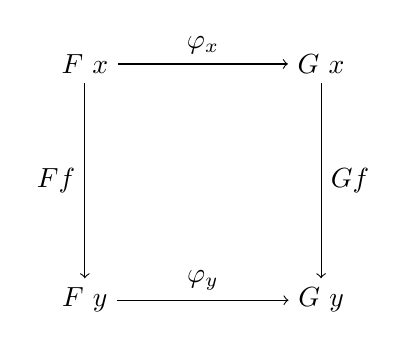
\begin{tikzpicture}[node distance=3cm and 1cm]
  \node (Px)               {$F~x$};
  \node (Qx) [right of=Px] {$G~x$}
    edge [<-] node[above] {$\varphi_x$} (Px);
  \node (Py) [below of=Px] {$F~y$}
    edge [<-] node [left] {$Ff$} (Px);
  \node      [below of=Qx] {$G~y$}
    edge [<-] node [above] {$\varphi_y$} (Py)
    edge [<-] node [right] {$Gf$} (Qx);
\end{tikzpicture}
\end{center}
commutes.

For two functions $f, g : C \to D$ regarded as functions between the associated groupoids, this becomes a family of paths $$\varphi_x : f~x =_D g~x.$$ The naturality condition of the above diagram becomes the condition that, for any path $p : x = y$,
$$(\ap f~p) \cdot \varphi_y = \varphi_x \cdot (\ap g~p)$$
and one can show that it holds for all
$$\varphi : \Pi_{(x : C)}~f~x =_D g~x.$$ Indeed, by path induction, assume $p$ is $\idp$ and $y$ is $x$. The path now reduces to $$\varphi_x = \varphi_x$$ which is inhabited by $\idp$.

Other basic type formers can be viewed as categorical constructions in this 2-category $\Gpd$. The product of types becomes the product of groupoids, with morphisms taken point-wise. The coproduct of types becomes the coproduct of groupoids. The path space here is only non-empty when both values are $\inl$ or $\inr$ and in this case matches the underlying one. $\Pi$ types/$\Sigma$ types become ends/coends, defined in \Cref{sec:cattheory}.

\chapter{Presheaves}

\section{$\mathcal{U}$-Presheaves}

In category theory, a presheaf on a category $\mathbb{C}$ is a functor $\mathbb{C}^{\mathrm{op}} \to \mathbf{Set}$. As for a groupoid $\mathbb{G} \cong \mathbb{G}^{\mathrm{op}}$, without loss of generality, under our interpretation, $\mathbb{C}^{\mathrm{op}}$ becomes $(C , \mathrm{Id}_C)$ and $\mathbf{Set}$ can be taken, in the first instance, to be $\mathcal{U}$. $\mathcal{U}$ is being treated as a category here, so the definition of functors between groupoids from \Cref{chap:interp} does not apply.

Instead, we want a mapping on objects
$$c : C \mapsto F~c : \mathcal{U}$$
and a mapping on morphisms
$$(c = c') \mapsto (F~c \to F~c').$$ In homotopy type theory we can define the function
$$\coe : (c = c') \to c \to c'$$
using path induction as
$$\coe\,\idp\,c \defeq c.$$
In combination with $\ap$ this gives
$$\coe \circ \ap F : (c = c') \to F~c \to F~c'$$
as we need. This is such a common operation in homotopy type theory that it has its own name, $\transport$. Thus we consider functions $F : C \to \mathcal{U}$ as presheaves on $C$ and will write the type of presheaves on $C$ as $\widehat{C}$.

A natural transformation, $\theta : \mathrm{Nat}(P , Q)$, between two presheaves, $P , Q : \mathbb{C} \to \mathbb{D}$, is a family of morphisms, $$\theta_x : P~x \to Q~x,$$ such that for all $x , y \in \mathbb{C}$ and $f : x \to y$ the following diagram commutes.

\begin{center}
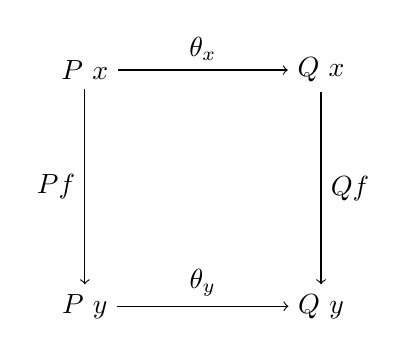
\begin{tikzpicture}[node distance=3cm and 1cm]
  \node (Px)               {$P~x$};
  \node (Qx) [right of=Px] {$Q~x$}
    edge [<-] node[above] {$\theta_x$} (Px);
  \node (Py) [below of=Px] {$P~y$}
    edge [<-] node [left] {$Pf$} (Px);
  \node      [below of=Qx] {$Q~y$}
    edge [<-] node [above] {$\theta_y$} (Py)
    edge [<-] node [right] {$Qf$} (Qx);
\end{tikzpicture}
\end{center}

For $P , Q : \widehat{C}$, this translates directly to the $\Pi$ type $$\mathrm{Nat}(P,Q) \defeq \prod_{(c : C)} P~c \to Q~c.$$ For an element of this type to be natural it needs to satisfy, for all $p : x = y$, $$\theta_y \circ~\mathrm{transport}~P~p = \mathrm{transport}~Q~p~\circ~\theta_x.$$
This holds for all elements of the type $\mathrm{Nat}$ by path induction as, by the definition of $\mathrm{transport}$, we have $$\mathrm{transport}~P~\idp = \mathrm{id},$$ where $\mathrm{id}$ is the identity function and by the left and right unit laws of function composition we have to show $\theta_x = \theta_x$ which is inhabited by $\idp$.

\section{Yoneda}

The Yoneda functor, $Y : \mathbb{C} \to \widehat{\mathbb{C}}$, takes each object of $\mathbb{C}$ to the presheaf $$Y~c \defeq \mathbb{C}(c,-),$$ i.e. to the presheaf that for all $x \in \mathbb{C}$ returns the hom from $c$ to $x$. Our interpretation takes homs to identity types, which means that the Yoneda functor becomes $$Y~c~x \vcentcolon\equiv c = x.$$

The Yoneda Lemma states that given an object $c \in \mathbb{C}$, the set of natural transformations from $Y~c$ to some other presheaf $X$ is isomorphic to the set $X~c$, which in type theory becomes $$\mathrm{Nat}(Y~c , P) \simeq P~c.$$

Let us look at the Agda proof of the Yoneda Lemma to get an idea of the steps involved in formalisation.

{\small
\begin{verbatim}
yonedaLemma : ∀ (P : prshf i C) (c : C)
            → P c ≃ nat (yon c) P
yonedaLemma P c = equiv f g (λ b → λ= (λ x → λ= (f-g b x))) (λ _ → idp)

  where

    f : P c → nat (yon c) P
    f p x idp = p

    g : nat (yon c) P → P c
    g p = p c idp

    f-g : (b : nat (yon c) P) → (x : C) → (p : yon c x)
        → f (g b) x p == b x p
    f-g b x idp = idp
\end{verbatim}}

The proof looks like what one might write on paper. To show that this is an equivalence, it is enough to exhibit functions in each direction, \texttt{f} and \texttt{g}, and show that their compositions act like the respective identities.

\paragraph{Density Formula}

The density formula is related to the Yoneda Lemma and will be used in several proofs. It is defined as
$$P~c \simeq \Sigma_{(x : C)}~(P~x) \times (x = c)$$
The Agda proof is again very similar to pen and paper, defining an equivalence by giving functions in both directions and showing their compositions act as identities.

{\small
\begin{verbatim}
density : ∀ (P : prshf C) (c : C) → P c ≃ Σ C (λ x → (P x) × (x == c))
density P c = equiv f g f-g (λ _ → idp)

  where

    f : P c → Σ C (λ x → P x × (x == c))
    f p = (c , p , idp)

    g : Σ C (λ x → P x × (x == c)) → P c
    g (_ , q , idp) = q

    f-g : (b : Σ C (λ x → P x × (x == c))) → f (g b) == b
    f-g (_ , q , idp) = idp
\end{verbatim}}

\section{Cartesian Closure of $\widehat{C}$}

The type of presheaves on a type $C$, $\widehat{C}$, forms a category, with objects the elements of $\widehat{C}$ and homs, for presheaves $P, Q : \widehat{C}$, the natural transformations $\Nat(P,Q)$. Identities of type $\Nat(P,Q)$ are given by
$$\lambda\,c \to \id.$$
Composition of $\Nat$s, for $\psi : \Nat(Q,R)$ and $\phi : \Nat(P,Q)$, is given by
$$\lambda\,c \to \psi\,c \circ \phi\,c.$$
This satisfies the unit and associativity laws by the units and associativity of function composition.

The terminal object is the constantly $\top$ presheaf,
$$\lambda\,\_ \to \top.$$
For any other presheaf $P$, the terminal morphism is given by
$$\lambda\,c\,p \to \mathrm{unit},$$
and this is clearly unique.

The product of two presheaves $P , Q : \widehat{C}$ is taken point-wise, so $$(P \times Q)~c \defeq P~c \times Q~c.$$ This is a product if it satisfies
$$\Nat(P,Q \times R) \simeq \Nat(P,Q) \times \Nat(P,R).$$ The forward direction of this equivalence is
$$f\,\phi \defeq ((\lambda\,c\,p \to \pi_1\,(\phi\,c\,p)) , (\lambda\,c\,p \to \pi_2\,(\phi\,c\,p))),$$
and the backward direction is
$$g\,(\phi_1 , \phi_2)\,c\,p \defeq (\phi_1\,c\,p , \phi_2\,c\,p).$$
These are clearly inverse, so we have a product.

The exponential object for two presheaves is defined as $$(P \Rightarrow Q)~c \defeq (Y~c \times P) \Rightarrow Q.$$ This is an exponential if it satisfies
$$\Nat(P \times Q,R) \simeq \Nat(P,Q \Rightarrow R).$$
The forward direction of this equivalence is
$$f\,\phi\,c\,p\,(\idp , q) \defeq \phi\,c\,(p , q),$$
and the backward direction is
$$g\,\phi\,c\,(p , q) \defeq \phi\,c\,p\,c\,(\idp , q).$$
Again these are clearly inverse, so we have an exponential.

\section{Left Kan Extension}
\label{sec:lans}

% Talk about universality of this

Consider the following diagram
\begin{center}
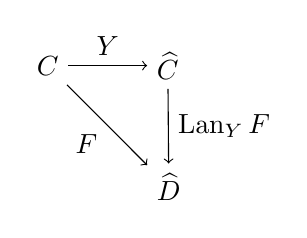
\begin{tikzpicture}
  \node (1) {$C$};
  \node (2) [right=of 1] {$\widehat{C}$}
    edge[<-] node[above] {$Y$} (1);
  \node (3) [below right=of 1] {$\widehat{D}$}
    edge[<-] node[below left] {$F$} (1)
    edge[<-] node[right] {$\Lan_Y F$} (2);
\end{tikzpicture}
\end{center}
The function $\Lan_Y F$ is the left Kan extension of the function $F$ along the Yoneda functor. This gives us a way to lift functions to act on presheaves. There is a general definition of the left Kan extension, but for our purposes it is enough to define it just for Yoneda. In this case the definition is
$$\Lan_Y F\,P\,d \defeq \Sigma_{(c : C)}\,P\,c \times F\,c\,d$$
using a coend which here is a $\Sigma$ type.

$\Lan_Y$ has many interesting properties that will be used when proving properties of species. The left Kan extension of the Yoneda functor is the identity function, which is proved by an application of the density formula,
$$\Lan_Y Y = \id.$$ The Yoneda functor composed with $\Lan_Y F$ gives back $F$,
$$\Lan_Y F \circ Y = F,$$ again proved using the density formula. The composition of two $\Lan_Y$s reduces to the $\Lan_Y$ of one $\Lan_Y$ composed with the first function,
$$\Lan_Y G \circ \Lan_Y F = \Lan_Y\,(\Lan_Y G \circ F),$$
which is proved by a simple permutation of the components of the $\Sigma$ type.

For $F : C \to \widehat{D}$ and $P , Q : \widehat{C}$, the action of $\Lan_Y$ on the coproduct of $P$ and $Q$ is given by
$$\Lan_Y F\,(\lambda\,c \to P\,c \sqcup Q\,c)\,d = \Lan_Y F\,P\,d \sqcup \Lan_Y F\,Q\,d.$$
This comes from,
\begin{align*}
&\quad\ \Lan_Y F\,(\lambda\,c \to P\,c \sqcup Q\,c)\,d \\
&\equiv \Sigma_{(c : C)}\,(P\,c \sqcup Q\,c) \times F\,c\,d \\
&\simeq (\Sigma_{(c : C)}\,P\,c \times F\,c\,d) \sqcup (\Sigma_{(c : C)}\,Q\,c \times F\,c\,d) \\
&\equiv (\Lan_Y F\,P\,d) \sqcup (\Lan_Y F\,Q\,d).
\end{align*}
% This is a universal extension in that for any other function $G : \hat{A} \to \hat{B}$ making the diagram commute factors

\section{Day Convolution}
\label{sec:dayconv}

Given a category, $\mathbb{C}$, that has a monoidal structure, Day Convolution extends the structure to presheaves on $\mathbb{C}$. The associative operation, $\daytensor$, is defined using two coends as
$$(P \daytensor Q)~c \defeq \int^{(c_1 , c_2 \in \mathbb{C})} P~c_1 \times Q~c_2 \times \mathbb{C}(c_1 \otimes c_2 , c).$$
Under our interpretation coends are $\Sigma$ types and homs are path spaces, leading to the definition
$$(P \daytensor Q)~c \defeq \Sigma_{(c_1 : C)}\Sigma_{(c_2 : C)}~P~c_1 \times Q~c_2 \times (c = c_1 \otimes c_2).$$

The identity presheaf for this operation makes reference to the identity for the underlying structure, the identity being defined as $$\dayid \defeq Y\,e.$$

To form a commutative monoid these need to be accompanied by proofs of the left and right unit laws, the associativity law, and the commutativity law. We will look in detail at the proof of the left unit law, first as a pen-and-paper proof and then in Agda. The left unit law for a monoid states that
$$\Pi_{(c : C)}~e \otimes c = c$$
which for the Day Convolution becomes
$$\Pi_{(P : \widehat{C})}~\dayid \daytensor P = P.$$ By function extensionality and the univalence axiom it is enough to show
$$\Pi_{(P : \widehat{C})}\Pi_{(c : C)}~(\dayid \daytensor P)~c \simeq P~c.$$ Taking arbitrary $P$ and $c$ we have
\begin{align*}
  (\dayid \daytensor P)~c &\equiv \Sigma_{(c_1 : C)}\Sigma_{(c_2 : C)}~(c_1 = e) \times P~c_2 \times (c = c_1 \otimes c_2) \\
  &\simeq \Sigma_{(c_2 : C)}~P~c_2 \times \Sigma_{(c_1 : C)}~(c = c_1 \otimes c_2) \times (c_1 = e) &&\text{(commutativity of $\Sigma$)} \\
  &\simeq \Sigma_{(c_2 : C)}~P~c_2 \times (c = e \otimes c_2) &&\text{(density formula)} \\
  &\simeq \Sigma_{(c_2 : C)}~P~c_2 \times (c = c_2) &&\text{(left unit law for $\otimes$)} \\
  &\simeq \Sigma_{(c_2 : C)}~P~c_2 \times (c_2 = c) &&\text{(symmetry of paths)} \\
  &\simeq P~c &&\text{(density formula)}
\end{align*}

The Agda proof below gives a representative example of `equational reasoning' proofs in Agda. Equational reasoning proofs chain together several steps of an equivalence or equality and include the types of each step for clarity.

{\small
\begin{verbatim}
ø-unit-l : (P : prshf C) → ∀ c → (ı ø P) c ≃ P c
ø-unit-l P c =

  (ı ø P) c

    ≃⟨ perm ⟩

  Σ C (λ c₂ → P c₂ × Σ C (λ c₁ → (c == (c₁ ⊗ c₂)) × (c₁ == e)))

    ≃⟨ Σ-emap-r (λ c₂ →
        ×-emap-r
          (P c₂)
          ((density (λ p → c == (p ⊗ c₂)) e)⁻¹)) ⟩

  Σ C (λ c₂ → P c₂ × (c == (e ⊗ c₂)))

    ≃⟨ Σ-emap-r (λ c₂ →
        ×-emap-r
          (P c₂)
          (coe-equiv (ap (c ==_) ⊗-unit-l))) ⟩

  Σ C (λ c₂ → P c₂ × (c == c₂))

    ≃⟨ Σ-emap-r (λ c₂ →
        ×-emap-r
          (P c₂)
          (!-equiv)) ⟩

  Σ C (λ c₂ → P c₂ × (c₂ == c))

    ≃⟨ (density P c)⁻¹ ⟩

  P c

    ≃∎
\end{verbatim}}

Each step of the proof corresponds to one step of the pen-and-paper proof. The only difference in the formalisation is that the justifications have to specify exactly what context they are being applied in and how exactly they are being applied.

We have a couple of results about monoid homomorphisms with respect to Day Convolution. Firstly the Yoneda functor is a homomorphism, because applied to $e$ it returns $\dayid$ and applied to $x \otimes y$, we can show that we get $Y\,x \daytensor Y\,y$.

Secondly, for any two monoids, $C$ and $D$, and a monoid homomorphism, $F : C \to \widehat{D}$, where the monoid of the codomain is given by Day Convolution, we have that $\Lan_Y F$ is also a monoid homomorphism with respect to Day Convolution in both the domain and codomain. The unit law is proved using a single application of the density formula and the unit law for $F$. The multiplication law is proved similarly with an application of the density formula and the multiplication law for $F$, however this time requires permutations of the components of the $\Sigma$ type before and after these are applied.

\section{$\mathcal{U}_n$-Presheaves}

The definitions of the previous four sections were for $\mathcal{U}$-valued presheaves, but as mentioned in \Cref{chap:interp} we will have to restrict to $\hProp$ or $\hSet$-valued presheaves later on. We therefore reformalise the results from above in the context of $\mathcal{U}_n$-valued presheaves. This will require projecting out underlying types from the $\mathcal{U}_n$ as well as carrying around proofs of truncation levels.

After redefining the type of presheaves we need to redefine natural transformations between presheaves to be truncated. This leads to the definition, for $C : \mathcal{U}_{\Suc\,(\Suc n)}$,
$$\Nat(P,Q) \defeq ((\Pi_{(c : C)}\,\pi_1\,(P\,c) \to \pi_1\,(Q\,c)) , \mathrm{\Pi\mhyphen level}\,(\lambda\,c \to \mathrm{\to\mkern-4mu\mhyphen level} (\pi_2\,(Q\,c)))).$$
This is absolutely typical of the changes that have to be made to the rest of the constructs we define. We add first projection functions to the types and use the second projections to reason about the truncation level.

\paragraph{Yoneda}

For some $C : \mathcal{U}_{\Suc\,(\Suc n)}$ we can redefine the Yoneda functor to return a $\mathcal{U}_{\Suc n}$-valued presheaf as
$$Y\,c\,x \defeq ((c = x) , (\pi_2\,C)\,c\,x).$$ The proofs of the Yoneda lemma and the density formula remain largely unchanged once the types have been projected out.

\paragraph{Left Kan Extension}

The definition of the left Kan extension was a sigma type whose first component was of type $C$. Our $C$ is now of type $\mathcal{U}_{\Suc\,(\Suc n)}$, but the result should have type $\mathcal{U}_{\Suc n}$. Therefore we need to use the truncation operation, defined in \Cref{sec:HoTT} to restrict the truncation level of the result. The new definition is
$$\Lan_Y F\,P\,d \defeq \| \Sigma_{(c : C)}\,P\,c \times F\,c\,d \|_{\Suc n}.$$
The proofs of the properties of $\Lan$s now need to be modify to take this into account. The are all modified similarly to the proof of Day Convolution that we will look at in detail.

\paragraph{Day Convolution}

Again the definition contains a component of type $C$, so we need to use truncation. This leads to the definition
$$(P \daytensor Q)~c \defeq \left\| \Sigma_{(c_1 : C)}\Sigma_{(c_2 : C)}~P~c_1 \times Q~c_2 \times (c = c_1 \otimes c_2)\right\|_{(\Suc n)}.$$

The change is reflected in the Agda proof, which now becomes
{\small
\begin{verbatim}
ø-unit-l : (P : prshf i C) → ∀ x → fst ((ı ø P) x) ≃ fst (P x)
ø-unit-l P x =

  fst ((ı ø P) x)

      ≃⟨ Trunc-emap (S n) perm ⟩

  Trunc
    (S n)
    (Σ C (λ c₂ → fst (P c₂) × Σ C (λ c₁ → (x == (c₁ ⊗ c₂)) × (c₁ == e))))

      ≃⟨ Trunc-emap (S n)
          (Σ-emap-r (λ c₂ →
           ×-emap-r
            (fst (P a₂))
            ((density (λ c → ((x == (c ⊗ c₂)) , p x (c ⊗ c₂))) e)⁻¹))) ⟩

  Trunc (S n) (Σ C (λ c₂ → fst (P c₂) × (x == (e ⊗ c₂))))

      ≃⟨ Trunc-emap (S n)
          (Σ-emap-r (λ c₂ →
           ×-emap-r
            (fst (P c₂))
            (!-equiv ∘e coe-equiv (⊗-unit-l |in-ctx (λ p → x == p))))) ⟩

  Trunc (S n) (Σ C (λ c₂ → fst (P c₂) × (c₂ == x)))

      ≃⟨ Trunc-emap (S n) (density P x)⁻¹ ⟩

  Trunc (S n) (fst (P x))

      ≃⟨ unTrunc-equiv (fst (P x)) (snd (P x)) ⟩

  fst (P x)

      ≃∎
\end{verbatim}}

Each step is now performed within a $\mathrm{Trunc\mhyphen emap}~(\Suc n)$ which uses an equivalence within the truncation. Then there is an additional last step that removes the truncation, which is allowed because $P$ is a $\mathcal{U}_{(\Suc n)}$-valued presheaf.

% The first step applies a permutation, not defined here, to the $\Sigma$ type within the truncation. This is an example of using an ``emap'', which builds an equivalence between two values of some type by using an equivalence between two subparts of the type. In other words the equivalence can be applied in some context, such as a truncation or a $\Sigma$ type.
%
% The second step uses more ``emap''s to apply the density formula deep within the structure of the type. The third step uses the left unit law of the underlying monoid structure and reverses the direction of the equality. The fourth step applies the density formula a second time, this time leaving us with the result, but inside a truncation. However, \texttt{P} is an \texttt{(S n)-Type}-valued presheaf, so the truncation has no effect and can be removed in the final step.

\section{Agda Formalisation}

\subsection{$\mathcal{U}$-presheaves}

\begin{center}
\begin{tabular}{ll}
  Concept & Agda Name \\
  \hline
  $\mathcal{U}$-presheaf & \texttt{prshf} \\
  $\Nat$ & \texttt{nat} \\
\end{tabular}
\end{center}

\subsection{Yoneda}

\begin{center}
\begin{tabular}{ll}
  Concept & Agda Name \\
  \hline
  Yoneda Functor & \texttt{yon} \\
  Yoneda Lemma & \texttt{yoneda-lemma} \\
  Yoneda Embedding & \texttt{yoneda-embedding} \\
  Density Formula & \texttt{density} \\
\end{tabular}
\end{center}

\subsection{Cartesian Closure of $\widehat{C}$}

\begin{center}
\begin{tabular}{ll}
  Concept & Agda Name \\
  \hline
  $\Nat$ Identity & \texttt{id$_\texttt{n}$} \\
  $\Nat$ Composition & $\_\circ_\texttt{n}\_$ \\
  Presheaf Product & \texttt{prod} \\
  Product Equivalence & \texttt{prod-equiv} \\
  Presheaf Sum & \texttt{sum} \\
  Sum Equivalence & \texttt{sum-equiv} \\
  Presheaf Exponential & $\_\Rightarrow\_$ \\
  Exponential Equivalence & \texttt{$\Rightarrow$-curry} \\
  Terminal Presheaf & \texttt{$\top$-prshf} \\
  Terminal Universal Morphism & \texttt{$\top$-prshf-morphism} \\
  Terminal Universal Uniqueness & \texttt{$\top$-prshf-uniqueness} \\
  Initial Presheaf & \texttt{$\bot$-prshf} \\
  Initial Universal Morphism & \texttt{$\bot$-prshf-morphism} \\
  Initial Universal Uniqueness & \texttt{$\bot$-prshf-uniqueness} \\
\end{tabular}
\end{center}

\subsection{Left Kan Extension}

\begin{center}
\begin{tabular}{ll}
  Concept & Agda Name \\
  \hline
  Left Kan Extension & \texttt{lan-y} \\
  $\Lan_Y$ of Yoneda & \texttt{lan-y-yon} \\
  $\Lan_Y$ Composed with Yoneda & \texttt{lan-y-$\circ$-yon} \\
  Composition of $\Lan_Y$s & \texttt{lan-y-$\circ$} \\
  $\Lan_Y$ Composed with Coproduct & \texttt{lan-y-$\sqcup$} \\
\end{tabular}
\end{center}

\subsection{Day Convolution}

\begin{center}
\begin{tabular}{ll}
  Concept & Agda Name \\
  \hline
  Commutative Monoid & \texttt{IsCommMonoid} \\
  Day Tensor & $\_\daytensor\_$ \\
  Day Unit & $\dayid$ \\
  Day Unit Left & \texttt{$\daytensor$-unit-l} \\
  Day Unit Right & \texttt{$\daytensor$-unit-r} \\
  Day Associativity & \texttt{$\daytensor$-assoc} \\
  Day Commutativity & \texttt{$\daytensor$-comm} \\
  Day Convolution & \texttt{day-convolution} \\
  Yoneda Homomorphism Unit & \texttt{yon-hom-unit} \\
  Yoneda Homomorphism Mult & \texttt{yon-hom-mult} \\
  $\Lan_Y$ Homomorphism Unit & \texttt{lan-y-hom-unit} \\
  $\Lan_Y$ Homomorphism Mult & \texttt{lan-y-hom-mult} \\
\end{tabular}
\end{center}

\subsection{$\mathcal{U}_n$-Presheaves}

All the of the concepts of the last five subsections have also been implemented for $\mathcal{U}_n$-presheaves.

\chapter{Free Symmetric Monoid}

For a small category $\mathbb{C}$, $\SM~\mathbb{C}$ is its free strict symmetric-monoidal completion. This can be explicitly defined as the category whose objects are finite sequences $\Lbrbrak c_i \Rbrbrak_{i = 1,\dots,n}$ of objects of $\mathbb{C}$ and whose homs from $\Lbrbrak c_i \Rbrbrak_{i = 1,\dots,n}$ to $\Lbrbrak c'_j \Rbrbrak_{j = 1,\dots,m}$ are only non-empty when $n = m$ and consist of pairs of a bijection $\sigma \in \mathlarger{\mathlarger{\mathlarger{\sigma}}}_n$ and a sequence of maps $\Lbrbrak f_i : c_i \to c'_{\sigma i} \Rbrbrak_{i = 1,\dots,n}$ in $\mathbb{C}$. The translation of this $\SM$ operator into the type theory is a significant focus of this project.

This section discusses our first attempt at formalisation. The idea is to take the type $\List C$, in which elements are ordered sequences of elements of $C$ and, to get the morphisms as the bijections between these sequences, take the quotient of this type by the relation of list permutations. Taking the quotient requires the use of Higher Inductive Types (HITs).

\section{Higher Inductive Types}

HITs are one of homotopy type theory's key contributions and most active research areas. Type theory uses the relatively simple framework of inductive types to reason about inductive structures. Although simple, inductive types are powerful reasoning tools, because one can automatically extract induction principles directly from their definitions.

Homotopy theory uses a similar idea of inductively defined spaces. These are defined by not only a collection of points but also a collection of paths or even higher paths. When this idea is taken into homotopy type theory, where paths are now identities, one can extract induction principles for these also. This provides a new way of understanding standard constructions of homotopy theory.

For a given HIT there are two forms of induction principle: the elimination rule, for the dependent case, and the simpler recursion rule, for the non-dependent case. The latter is usually defined in terms of the former. These allow the definition of functions where the domain is a HIT and are necessary because one cannot pattern match on, or deconstruct HITs otherwise.

\section{Quotients}
\label{sec:quotients}

Given a type $C$ and a relation, $R : C \to C \to \mathcal{U}$, on this type we can form the quotient of $C$ by this relation. This can be defined as the following HIT
\begin{equation}
\label{eqn:quot}
\begin{array}{l}
  \mathtt{HIT}~\Quot \defeq \\
  \quad \q : C \to \Quot \\
  \quad \rel : \Pi_{(x,y : C)}~R~x~y \to \q x = \q y \\
\end{array}
\end{equation}
There is a collection of points $\q c$, with one point for each point $c : C$. However, if two points are related according to the relation $R$, then they are considered equal in the type $\Quot$. This is actually a quotient by $R^*$, the reflexive-symmetric-transitive closure of $R$. It is reflexive because we always have $\idp : \q x = \q x$. It is symmetric because if we have $r : R~x~y$, but not $R~y~x$ in the relation, we still get $!~(\rel r) : \q y = \q x$. Transitivity similarly comes from path composition.

The elimination principle can be extracted from the type above by forcing the resulting property to reflect the structure of the HIT. Specifically, it has type
$$
\begin{array}{rl}
  \mathrm{elim}_{\Quot} :& \Pi_{(P : \Quot \to \mathcal{U})} \\ &\Pi_{(\qs : \Pi_{(c :C)}~P~(\q c))} \\ & (\Pi_{(x , y : C)}\Pi_{(r : R~x~y)} \to \qs x = \qs y~[P \downarrow \rel x~y~r]) \\ &\to \Pi_{(p : \Quot)}~P~p,
\end{array}
$$
which says that to define a dependent function from $\Quot$ to some property $P : \Quot \to \mathcal{U}$ we need a point in the resulting property for every point in $\Quot$ and a dependent path over every $\rel$ path.

This simplifies, in the non-dependent case, to the recursion principle,
$$
\begin{array}{rl}
  \mathrm{rec}_{\Quot} :& \Pi_{(D : \mathcal{U})} \\ &\Pi_{(\qs : C \to D)} \\ & (\Pi_{(x , y : C)}~R~x~y \to \qs x = \qs y) \\ &\to \Quot \to D.
\end{array}
$$

\paragraph{Set Quotients}

In \Cref{sec:hsetmodel} we will define a model of the $\SM$ construction for $\hSet$s, but to do this the result of applying $\SM$ should be an $\hSet$. \Cref{eqn:quot} says nothing about the higher path structure of the resulting type, so there is no guarantee that it will be a set. Therefore the following HIT is more appropriate
\begin{equation}
\label{eqn:setquot}
\begin{array}{l}
  \mathtt{HIT}~\SetQuot \defeq \\
  \quad \q : C \to \SetQuot \\
  \quad \rel : \Pi_{(x,y : C)}~R~x~y \to \q x = \q y \\
  \quad \mathrm{SetQuot\mhyphen is\mhyphen set} : \isset \SetQuot
\end{array}
\end{equation}
The extra constraint of type $\isset$, defined in \Cref{sec:HoTT}, ensures that all path structure above the set level is collapsed and the resulting type can be treated as a set. This change influences the elimination and recursion principles. The first becomes
$$
\begin{array}{rl}
  \mathrm{elim}_{\SetQuot} :& \Pi_{(P : \SetQuot \to \mathcal{U})} \\ &\Pi_{(\qs : \Pi_{(c :C)}~P~(\q c))} \\ & (\Pi_{(x , y : C)}\Pi_{(r : R~x~y)} \to \qs x = \qs y~[P \downarrow \rel x~y~r]) \\ &\to (\Pi_{(c : C)}~\isset P~c) \\ &\to \Pi_{(p : \SetQuot)}~P~p
\end{array}
$$
adding a proof of $\isset$ for every resulting property and the second becomes
$$
\begin{array}{rl}
  \mathrm{rec}_{\SetQuot} :& \Pi_{(D : \mathcal{U})} \\ &\Pi_{(\qs : C \to D)} \\ & (\Pi_{(x , y : C)}~R~x~y \to \qs x = \qs y) \\ &\to \isset D \\ &\to \SetQuot \to D
\end{array}
$$
adding a proof of $\isset D$.

\paragraph{Groupoid Quotients}

In \Cref{sec:hgpdmodel} we will extend the $\SM$ model to further work for $\hGpd$s, which again requires a change to the quotient. The type will be restricted to being a groupoid rather than a set, which means there will be more path structure. Modifying \Cref{eqn:setquot} below to use $\isgpd$, defined in \Cref{sec:HoTT}, gives one definition of a quotient at the groupoid level, but it is not general enough for our purposes. This definition would again be quotienting by $R^*$, but this time, because we are working with a groupoid, the reflexivity and transitivity paths do not necessarily coincide with the ones that $R$ may already have. To generalise, given an $R$ along with $$\Rrefl : \Pi_{(c : C)}~R~c~c,$$ a proof of reflexivity, and $$\Rtrans : \Pi_{(x , y , z : C)}~R~x~y \to R~y~z \to R~x~z,$$ a proof of transitivity, we want to force the former to coincide with $\idp$ and the latter to coincide with $\cdot$. This leads to the following HIT
\begin{equation}
\label{eqn:setquot}
\begin{array}{l}
  \mathtt{HIT}~\GpdQuot \defeq \\
  \quad \q : C \to \GpdQuot \\
  \quad \rel : \Pi_{(x,y : C)}~R~x~y \to \q x = \q y \\
  \quad \relidp : \Pi_{(c : C)} \rel c~c~(\Rrefl c) = \idp \\
  \quad \reldot : \Pi_{(x , y, z : C)}\Pi_{(r : R~x~y)}\Pi_{(r' : R~y~z)} \rel x~y~r \cdot \rel y~z~r' = \rel x~z~(\Rtrans r~r') \\
  \quad \mathrm{GpdQuot\mhyphen is\mhyphen gpd} : \isgpd \GpdQuot
\end{array}
\end{equation}

We note that one does not need to add symmetry, which would be given by
$$\Pi_{(x,y : C)}\Pi_{(r : R\,x\,y)}\,! (\rel x\,y\,r) = \rel y\,x\,(\Rsym r)$$
because it can be derived from the other two. We have
\begin{align*}
  \rel x\,y\,r \cdot ! (\rel x\,y\,r) &= \idp \\
  &= \rel x\,x\,(\Rrefl x) \\
  &= \rel x\,x\,(\Rtrans r\,(\Rsym r)) \\
  &= \rel x\,y\,r \cdot \rel y\,x\,(\Rsym r)
\end{align*}
and then
\begin{align*}
  ! (\rel x\,y\,r) &= ! (\rel x\,y\,r) \cdot \rel x\,y\,r \cdot ! (\rel x\,y\,r) \\
  &= ! (\rel x\,y\,r) \cdot \rel x\,y\,r \cdot \rel y\,x\,(\Rsym r) \\
  &= \rel y\,x\,(\Rsym r).
\end{align*}

The elimination and recursion principles need to reflect these new paths. The elimination principle becomes
$$
\begin{array}{rl}
  \mathrm{elim}_{\GpdQuot} :& \Pi_{(P : \GpdQuot \to \mathcal{U})} \\
  &\Pi_{(\qs : \Pi_{(c : C)}\,P\,(\q c))} \\
  &\Pi_{(\rels : \Pi_{(x , y : C)}\Pi_{(r : R\,x\,y)} \to \qs x = \qs y\,[P \downarrow \rel x\,y\,r])} \\
  & (\Pi_{(c : C)} \rels c~c~(\Rrefl c) = \idp^d~[ (\lambda p \to \qs c = \qs c~[P \downarrow p]) \downarrow \relidp c]) \\
  &\to (\Pi_{(x, y, z : C)}\Pi_{(r : R~x~y)}\Pi_{(r' : R~y~z)} \\
  & \quad\to \rels x~y~r \cdot \rels y~z~r' = \rels x~z~(\Rtrans r~r') \\
  & \quad\quad[(\lambda p \to \qs x = \qs z~[P \downarrow p]) \downarrow \reldot x~y~z~r~r'] \\
  &\to (\Pi_{(c : C)}~\isgpd P~c)) \\
  &\to \Pi_{(p : \GpdQuot)}~P~p
\end{array}
$$
This is quite complex, but can be derived mechanically from the definition of the HIT. Compared to the elimination principle for $\SetQuot$ there are two new families of dependent paths, lying over $\relidp$ and $\reldot$ respectively. Again this simplifies to the recursion principle
$$
\begin{array}{rl}
  \mathrm{rec}_{\GpdQuot} :& \Pi_{(D : \mathcal{U})} \\
  &\Pi_{(\qs : C \to D)} \\
  &\Pi_{(\rels : \Pi_{(x , y : C)}\,R\,x\,y \to \qs x = \qs y)} \\
  & (\Pi_{(c : C)} \rels c~c~(\Rrefl c) = \idp) \\
  &\to (\Pi_{(x, y, z : C)}\Pi_{(r : R~x~y)}\Pi_{(r' : R~y~z)} \\
  & \quad\to \rels x~y~r \cdot \rels y~z~r' = \rels x~z~(\Rtrans r~r')) \\
  &\to \isgpd D \\
  &\to \GpdQuot \to D
\end{array}
$$
which says that to define a function $\GpdQuot \to D$ we need to show that $D$ is a groupoid and further that $\qs$ preserves the structure of the relation, i.e. relates the appropriate elements and has reflexivity and transitivity.

The computation of these HITs is defined in Agda using a rewrite rule. For quotients the rule says
$$\mathrm{elim}_{\GpdQuot} \dots (\q c) \mapsto \qs c$$
where $\dots$ represents the arguments to the elimination rule.

\section{List Permutations}

A list permutation is any reordering of a list of elements that preserves all the elements. This can be seen as a bijection between two lists. The underlying type of sequences that we will use for the $\SM C$ construction is that of $\List C$. We then want the path space to contain bijections between these lists, so we want to define list permutations as a relation that can be used with the quotient.

To define list permutations we will need a couple of auxiliary definitions. The first is the predicate of list membership $\in$ which for elements $c , c' : C$ and a list $l : \List C$ has constructors
$$\here : c == c' \to c' \in (c :: l)$$
and
$$\there : c' \in l \to c' \in (c :: l).$$
These act as an index into the list $c :: l$ giving a position for the element $c'$ as a sequence of $\there$s and a final $\here$. The second is the $\remove$ function
$$\remove : \Pi_{(x : C)}\Pi_{(xs : \List C)}~x \in xs \to \List C$$
which traverses the list following the sequence of $\there$s and then removes the element that corresponds to the $\here$.

Using these, we define list permutations to be the inductive relation
\begin{align*}
&\mathbf{data}\,\ListPerm : \List C \to \List C \to \mathcal{U}\,\mathbf{where} \\
  &\quad\lpnil : \ListPerm \nil \nil \\
  &\quad\lpcons : \Pi_{\{x : C\}}\Pi_{\{xs , xs' : \List C\}}\Pi_{(e : x \in xs')}\,\ListPerm xs\,(\remove xs'\,e) \to \ListPerm\,(x :: xs)\,xs' \\
\end{align*}
In the base case the empty list is a permutation of itself. In the inductive case, the list $x :: xs$ is a permutation of the list $xs'$ if $x \in xs'$ and $xs$ is a permutation of $xs'$ with $x$ removed. This ensures that each element of one list appears exactly once in the other.

List permutations form an equivalence relation between lists on a type. Therefore they satisfy reflexivity,
$$\mathrm{ListPerm\mhyphen is\mhyphen refl} : \Pi_{(c : \List C)}~\ListPerm c~c,$$
symmetry,
$$\mathrm{ListPerm\mhyphen is\mhyphen sym} : \Pi_{(x , y : \List C)}~\ListPerm x~y \to \ListPerm y~x,$$
and transitivity,
$$\mathrm{ListPerm\mhyphen is\mhyphen trans} : \Pi_{(x , y , z : \List C)}~\ListPerm x~y \to \ListPerm y~z \to \ListPerm x~z.$$

Reflexivity is simple. For an empty list we have $\lpnil$. For a list $x :: xs$ we apply $\lpcons$ to $\here \idp$ and an inductive call to reflexivity. This is the identity permutation on a list.

Symmetry, corresponding to inverse permutations, is more involved. Consider the cases for an input $\sigma$. For $\sigma \equiv \lpnil$ we of course have $\lpnil$. For $\sigma \equiv \lpcons\,(\here \idp)\,\sigma'$ we have $\lpcons\,(\here \idp)\,(\mathrm{ListPerm\mhyphen is\mhyphen sym}\,\sigma')$. In the case of $\sigma \equiv \lpcons\,(\there e)\,\sigma'$ we have to do more. The permutation will look something like
\begin{center}
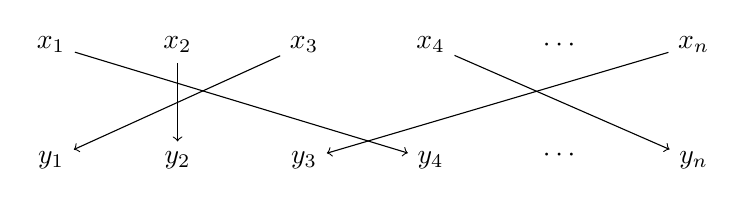
\begin{tikzpicture}
  \node (1) {$x_1$};
  \node (2) [right=of 1] {$x_2$};
  \node (3) [right=of 2] {$x_3$};
  \node (4) [right=of 3] {$x_4$};
  \node (5) [right=of 4] {$\cdots$};
  \node (6) [right=of 5] {$x_n$};
  \node (7) [below=of 1] {$y_1$}
    edge[<-] (3);
  \node (8) [below=of 2] {$y_2$}
    edge[<-] (2);
  \node (9) [below=of 3] {$y_3$}
    edge[<-] (6);
  \node (10) [below=of 4] {$y_4$}
    edge[<-] (1);
  \node (11) [below=of 5] {$\cdots$};
  \node (12) [below=of 6] {$y_n$}
    edge[<-] (4);
\end{tikzpicture}
\end{center}
and we want to define the inverse permutation, meaning we need to give a mapping for $y_1$. Notice that if we remove the pair $(x_1 , y_4)$, then the mapping for $x_2$ is a $\there$. Then, removing the pair $(x_2 , y_2)$, the mapping for $a_3$ is a $\here$. In general, to find the index for $y_1$ we count the distance to the first $\here$ value in the permutation, using the function $\firsthere$. Then the rest of the permutation should be a recursive call, applying symmetry to the permutation with the pair $(x_3 , y_1)$ removed. To remove this pair the indices of the first two pairs should be reduced. This is done using the $\remfirsthere$ function. The whole definition becomes $$\lpcons\,(\firsthere \sigma)\,(\mathrm{ListPerm\mhyphen is\mhyphen sym}\,(\remfirsthere \sigma)).$$

Finally transitivity, which corresponds to composition of permutations and which we'll write $\sigma_2 \circ \sigma_1$. Intuitively we just need to join up the lines of diagrams like the ones above. However, formalising this concept was one of the significant challenges of this project. So we have $\sigma_1 : \ListPerm x\,y$ and $\sigma_2 : \ListPerm y\,z$. In the base case we have both permutations being $\lpnil$ and the result is of course $\lpnil$. The next simplest case is the one where $\sigma_1 \equiv \lpcons\,(\here \idp)\,\sigma_1'$ and $\sigma_2 \equiv \lpcons e\,\sigma_2'$ because here the resulting permutation is simply $\lpcons e\,(\sigma_2' \circ \sigma_1')$.

The remaining two cases have the first permutation as $\sigma_1 \equiv \lpcons\,(\there e)\,\sigma_1'$. In both cases the first argument to $\lpcons$ is the index got following the two indices. To calculate this value we have the function
$$\mathrm{\in\mkern-4mu\mhyphen ListPerm} : x \in xs \to \ListPerm xs\,ys \to x \in ys$$
such that $\mathrm{\in\mkern-4mu\mhyphen ListPerm}\,(\there e)\,\sigma_2$ gives us the index of the first element of $x$ in $z$. We want to call $\circ$ recursively and the second argument will be $\sigma_1$. We need to consider the two cases for the first argument separately.

For the first case we have $\sigma_2 \equiv \lpcons\,(\here \idp)\,\sigma_2'$. $\sigma_1$ had a $\there$ at the head, so we will not be removing the first value of the second list. Therefore, the first argument to $\circ$ starts with $\lpcons\,(\here \idp)$. Now the tail of this list has to remove the pair which was used to join the first element. This removal is the most complicated part of the algorithm, so we will not go into the details.

For the second case we have $\sigma_2 \equiv \lpcons\,(\there e)\,\sigma_2'$. We cannot guarantee that the result starts with the same $\there e$ this time, so we instead call the removal function on the whole lists. Again the details of this are omitted.

\section{hSet Model}
\label{sec:hsetmodel}

The definition of the free strict symmetric-monoidal completion given at the beginning of this chapter was for categories. Before trying to model this for our interpretation of types as groupoids, we will first look at modelling the set-theoretic version of the same construction. This corresponds to the finite-multiset construction on sets.

From the definition at the beginning of the chapter, the construction on categories had objects as finite sequences of objects of the underlying category, and homs as bijections between these sequences. We can view the category as a set by collapsing the homs to having at most one morphism. Now there will be morphisms between two objects if and only if there is a bijection between them. There will now be fully connected components, each of which corresponds to a multiset.

Working with multisets, we get the notion of the empty multiset, $\varnothing$, corresponding to an empty sequence, and the union of multisets, $\cup$, corresponding to concatenation of sequences. These are the unit and associative operation of a monoid. We also get the singleton multiset containing $c$, $[c]$, corresponding to a singleton sequence.

To be the \textit{free} construction the definition must have the corresponding universal property, which says that for every set $C$ and commutative monoid $M$, a function $f : C \to M$ uniquely extends to a function $f^\# : \SM~C \to M$ that is a monoid homomorphism, i.e. it satisfies the unit law $$f^\#~\varnothing = e$$ and the multiplication law $$f^\#~(x \cup y) = f^\#~x \otimes f^\#~y,$$ where $e$ is the unit of $M$ and $\otimes$ its commutative, associative operation, and further satisfies the singleton law
$$f^\#~[c] = f~c.$$ It should also satisfy a uniqueness property that for any other monoid homomorphism $h$ such that
$$h~[c] = f~c$$ we should have that $$h = f^\#.$$

The $\hSet$ model of this finite multiset construction is obtained as
$$\SM C = \operatorname{SetQuot}_{\List C}(\ListPerm C),$$ quotienting the type of lists on $C$ by the relation of list permutations. This formalisation makes it easy to define the empty multiset
$$\varnothing \defeq \q \nil$$ and the singleton $$[c] \defeq \q~(c :: \nil).$$

The next step is to define the union operation, which combines two values of $\mathrm{SM}~C$. Defining a function where the domain is a HIT requires the use of the associated induction principle. The union operation is non-dependent, so the definition uses the recursion rule for quotients defined above.
{\small
\begin{verbatim}
_∪_ : SM C → SM C → SM C
_∪_ =
  SM-rec
    (→-is-set SM-is-set)
    (λ x →
      SM-rec
        SM-is-set
        (λ y → qp[ x ++ y ])
        (λ r → quot-rel (ListPerm-cong-++-r x r)))
    (λ r →
      λ=
        (SM-elim
          (λ _ → =-preserves-set SM-is-set)
          (λ y → quot-rel (ListPerm-cong-++-l r y))
          (λ _ → prop-has-all-paths-↓ (SM-is-set _ _))))
\end{verbatim}}
Here the $\q$ from the quotient has become the operator $\mathtt{qp[\_]}$ and the $\rel$ has become $\mathtt{quot\mhyphen rel}$, because the set quotient was already defined in HoTT-Agda with these names.

The union operation is a function of two arguments, so the recursion principle needs to be used twice. For the first application, the result is a function type. Function types have the same level as their codomain, so the whole function is a set because $\SM$ produces a set. To define $\qs$ for this operation we use the recursion rule a second time, with the first argument already in scope. The result is $\SM C$, which is a set. The $\qs$ at this second level defines the actual functionality of the union operation, which is to append the two underlying lists and then apply the quotient.

The rest of the definition is the proofs $\rels$ for each level. The inner $\rels$ is a congruence condition that says
$$\Pi_{(x , y , z : \List C)}\Pi_{(r : \ListPerm~y~z)}~\ListPerm~(x \lapp y)~(x \lapp z).$$ The outer $\rels$ requires an application of the elimination rule because it involves a dependent path. This itself requires another $\rels$ proof, but this one is at the level above set, so follows trivially because $\mathrm{SM}$ is a set. This trivialisation of higher $\rels$ proofs was part of the motivation for starting with the set theoretic model.

Given a function $f : C \to M$ for a commutative monoid $M$, the universal property uniquely extends to a function $f^\# : \SM C \to M$. Functions from $\SM C$ are defined using the recursion principle by giving a function on the underlying list, $\qs : \List C \to D$. For this we define the function $\monfold : (C \to D) \to \List C \to D$ as
$$\monfold~f \defeq \mathrm{foldr}~(\lambda~x~m \to f~x \otimes m)~e$$
which applies $f$ to each element of the list and joins the results using $M$'s associative operation. This must come with an associated $\rels : \Pi_{(x , y : C)}~\ListPerm x~y \to \qs x = \qs y$, which we get using the function $$\monfoldconst : \Pi_{(f : C \to M)}\Pi_{(x , y : C)}~\ListPerm x~y \to \monfold f~x = \monfold f~y.$$
This leads to the following definition of the universal property
$$f^\# \defeq \mathrm{rec}_{\SM}~M~(\monfold f)~(\monfoldconst f).$$

Finally we show that this definition satisfies the necessary conditions. The unit law follows from the definitions of $\varnothing$ and $\monfold$, as
$$\monfold \nil \defeq e.$$ The singleton law again follows computationally, as
$$\monfold~(c :: \nil) \defeq f~c.$$ To prove the multiplication law we use the elimination rule twice, with the inner $\qs$ being the function
$$\mathrm{monoid\mhyphen fold\mhyphen is\mhyphen\mkern-3mu\lapp} : \Pi_{(x , y : \List C)}\monfold~(x \lapp y) = \monfold x \otimes \monfold y,$$ which performs induction on $x$. When $x$ is $\nil$, then this is simply the left unit law for the monoid. When $x$ is $x :: xs$ this reduces to showing
$$f~x \otimes \monfold~(xs \lapp y) = (f~x \otimes \monfold xs) \otimes \monfold y,$$ which requires a recursive call and an application of associativity of the monoid operation.

To prove uniqueness we use function extensionality and the elimination principle leaving us to show
$$\monfold f~x = h~(\q x)$$
Again we use induction on $x$. In the $\nil$ case we can use the unit law for $h$. In the $x :: xs$ case we have
\begin{align*}
 \monfold~(x :: xs) &= f~x \otimes h~(\q xs) &&\text{(induction)} \\
  &= h~[x] \otimes h~(\q xs) &&\text{($h$ singleton law)} \\
  &= h~\q~(x :: xs) &&\text{($h$ multiplication law)}
\end{align*}

So the definition does give the desired universal property. Using the universal property the $\SM$ construction can be seen as an endofunctor on $\hSet$. The action of the $\SM$ construction on morphisms can be defined in terms of the universal property. For a function $f : C \to D$, $$\SM~f \defeq ([\_] \circ f)^\#.$$

\section{hGpd Model}
\label{sec:hgpdmodel}

In the $\hSet$ model, for any two values $x, y : \SM C$ the path space $x = y$ is a proposition, so all paths are considered equal. This means that, considering $\SM C$ as a groupoid every hom contains either no morphisms or one morphism. This restriction removes non-trivial groupoid structure. It is worthwhile to extend the definition to $\hGpd$s using $\GpdQuot$ from \Cref{sec:quotients}.

Again this HIT allows us to construct the type $\SM C$ by applying it to the relation $\ListPerm$ over $C$, extended with reflexivity and transitivity,
$$\SM C \defeq \operatorname{GpdQuot}_{\List C}(\ListPerm).$$

This time, however, proofs of simple properties become highly involved. For example, in the definition of the union operation in the $\hSet$ model, we only had to define $\rels$ for the inner application of the recursion principle, getting the outer one for free. Now we have to further define $\relidps$ and $\reldots$ for the inner application, and $\rels$ for the outer application, getting only the last two paths for the outer application trivially.

% Talk about interesting differences in the proofs from set theoretic version

\section{Agda Formalisation}

\subsection{Quotients}

\begin{center}
\begin{tabular}{ll}
  Concept & Agda Name \\
  \hline
  Groupoid Quotient Elimination Principle & \texttt{GpdQuot-elim} \\
  Groupoid Quotient Recursion Principle & \texttt{GpdQuot-rec} \\
\end{tabular}
\end{center}

\subsection{List Permutations}

\begin{center}
\begin{tabular}{ll}
  Concept & Agda Name \\
  \hline
  $\remove$ & \texttt{remove} \\
  $\ListPerm$ & \texttt{ListPerm} \\
  $\ListPerm$ Reflexivity & \texttt{id-perm} \\
  $\firsthere$ & \texttt{first-here} \\
  $\remfirsthere$ & \texttt{remove-first-here} \\
  $\ListPerm$ Symmetry & \texttt{inv-perm} \\
  $\mathrm{\in\mkern-4mu\mhyphen ListPerm}$ & \texttt{$\in$-ListPerm} \\
  $\ListPerm$ Transitivity & $\_\circ_\texttt{p}\_$ \\
  $\ListPerm$ Concatenation & $\_\lapp_\texttt{p}\_$ \\
  $\ListPerm$ $\lapp$ Congruence Left & \texttt{ListPerm-cong-++-l} \\
  $\ListPerm$ $\lapp$ Congruence Right & \texttt{ListPerm-cong-++-r} \\
\end{tabular}
\end{center}

\subsection{$\hSet$ Model}
\label{subsec:setformal}

\begin{center}
\begin{tabular}{ll}
  Concept & Agda Name \\
  \hline
  $\SM$ & \texttt{SM} \\
  $\varnothing$ & $\varnothing$ \\
  $[\_]$ & \texttt{SM-$\top$} \\
  $\cup$ & $\_\cup\_$ \\
  Union Unit Left & \texttt{$\cup$-unit-l} \\
  Union Unit Right & \texttt{$\cup$-unit-r} \\
  Union Associativity & \texttt{$\cup$-assoc} \\
  Union Commutativity & \texttt{$\cup$-comm} \\
  $\SM$ Monoid & \texttt{SM-is-comm-monoid} \\
  $\monfold$ & \texttt{monoid-fold} \\
  $\monfoldconst$ & \texttt{monoid-fold-is-const} \\
  Universal Extension & \texttt{up} \\
  Universal Homomorphism Unit & \texttt{up-hom-unit} \\
  Universal Homomorphism Mult & \texttt{up-hom-mult} \\
  Universal Applied to Singleton & \texttt{up-hom-$\top$} \\
  Universal Uniqueness & \texttt{up-uniqueness} \\
  $\SM$ Functor on Morphisms & \texttt{SM-fmap}
\end{tabular}
\end{center}

\subsection{$\hGpd$ Model}

The $\hGpd$ model defines all the same concepts as the $\hSet$ model. However, due to the difficulty of coherence proofs at the groupoid level the definitions of the $\rels$ paths for the Universal Extension, Universal Homomorphism Mult, Universal Applied to Singleton, and Universal Uniqueness were left postulated.

\chapter{A Truncated Formalisation}

\section{Imposed Finiteness}

The first formalisation of the free symmetric-monoidal completion was based on lists over some type $C$. These lists are finite by construction. The desired morphisms, i.e. permutations between these lists, were added directly using the quotient HIT. Alternatively lists over $C$ can be described using some finite indexing type $I$ and a function $f : I \to C$, leading to the definition
$$\SM_0 C \defeq \Sigma_{(I : \mathcal{U})}~(I \to C) \times \Sigma_{(n : \mathbb{N})}~I \simeq \Fin n.$$

Unfortunately this definition doesn't quite work, because the path space does not have the correct structure. For this type, the path space contains not only equality of the underlying indexing types and functions, but also of the proof of finiteness. This forces the types to be finite in the same way, trivially restricting the path space. To get around this problem the proofs of finiteness need to be ignored. This can be achieved using propositional truncation, the truncation operation at level $-1$. Truncating the proof of finiteness means that two different proofs are always equal, so no longer affect the path space. The final definition becomes
$$\SM C \defeq \Sigma_{(I : \mathcal{U})}~(I \to C) \times \Sigma_{(n : \mathbb{N})}~\|I \simeq \Fin n\|.$$ This is based on the definition of finite universes in \citet{yorgey2014combinatorial} and generalises it for our purposes.

Again we can define the empty value and the singleton value, although they are no longer as simple as the previous formalisation. The empty value is
$$\varnothing \defeq (\bot, \botrec, 0, | \finempty |)$$
where $\bot$ is the empty type, $\botrec$ is the unique function from the empty type to $C$, and $\finempty$ is a proof that $\Fin 0$ is equivalent to the empty type. The singleton value is
$$[c] \defeq (\top, \lambda~\_ \to c, 1, | \finunit |)$$
where $\top$ is the unit type, and $\finunit$ is a proof that $\Fin 1$ is equivalent to the unit type. These clearly have the desired behaviour, because the empty value picks out no $C$ values and $[c]$ picks out the specific value $c$.

The union operation has type $\SM C \to \SM C \to \SM C$, so needs to combine two values of this $\Sigma$ type. Take two values of the type: $(I , i , m , ti)$ and $(J , j , n , tj)$. To combine the first components is to create a new indexing set containing all the values of the two initial ones. This can be done using the coproduct which corresponds to a disjoint union of the types. The indexing function now has to perform case analysis on a value of type $I \sqcup J$. When the value is in $I$ we want to apply $i$ and when it is in $J$, $j$. This can be written $[i,j]$. $I \sqcup J$ clearly has size $m + n$, so finally we have to combine the two proofs of finiteness. To do this we first have to show
$$\mathrm{\sqcup\mhyphen finite} : I \simeq \Fin m \to J \simeq \Fin n \to I \sqcup J \simeq \Fin\,(m + n).$$
This can then be turned into a function on truncated values using $\mathrm{Trunc\mhyphen fmap2},$ which has type
$$(C \to D \to E) \to \| C \| \to \| D \| \to \| E \|,$$ and uses the truncation recursion principle twice, then simply applies the supplied function inside a truncation. So the final definition is
$$(I , i , m , ti) \cup (J , j , n , tj) \defeq (I \sqcup J , [i , j] , m + n , \mathrm{Trunc\mhyphen fmap2}\,\mathrm{\sqcup\mhyphen finite}~ti~tj).$$

Showing that $\SM C$ forms a commutative monoid with unit $\varnothing$ and associative operation $\cup$ reduces to showing the commutative monoid laws for the monoid with unit $\bot$ and associative operation $\sqcup$ and for the monoid with unit $1$ and associative operation $+$.

% Maybe look at this in detail

We want to define the universal property for this truncated definition, but to do so we need to define a function $\SM C \to M$, where $M$ is a monoidal groupoid. The type $\SM C$ contains a truncated value and truncation is defined as a HIT. Therefore, to use this value we need to use an appropriate recursion principle. The next section discusses such a principle.

\section{Functions from Propositional Truncations}

The usual recursion principle for propositional truncation has the type,
$$(C \to D) \to \isprop D \to \| C \| \to D.$$
So to construct a function out of a propositional truncation, the result has to be a proposition. Any definition of the universal property for the truncated $\SM C$ will have to use the truncated equivalence stored inside it, but we would like the result to be a groupoid, not a proposition. Therefore this recursion principle is not strong enough to allow us to define the universal property in its full generality.

The intuition behind using truncated values is that the result should not leak information hidden by the truncation. For example if $C$ is a set and has the higher path $p =_{c =_C c'} p'$, any function that uses a value of $\| C \|$ should not allow the knowledge that this path exists to leak into the result type. One way to enforce this is to force the result type to have the same truncation level, as is done in the above recursion principle. However, there should be some functions that do not leak information and yet have higher level results, the obvious example being a constant function to a type of higher level.

Intuitively, not leaking information corresponds to not caring what the value is, only that it exists, so we might want for some function $f : C \to D$,
\begin{equation}
\label{eqn:wconst}
\Pi_{(c, c' : C)}~f~c = f~c'.
\end{equation}
We conjectured that we should be able to use this property and found that \citet{kraus2014general} had indeed proved the equivalence
$$(\| C \| \to D) \simeq \Sigma_{(f : C \to D)}~\iswconst f,$$ for $D$ a set, where $\iswconst$ is exactly the property above, called weak-constancy. This property is not enough for the groupoid case however. The following path is needed to force higher paths to behave correctly in the groupoid case,
\begin{equation}
\label{eqn:coh}
\iscoh f~c \defeq \Pi_{(x , y , z : C)}~c~x~y \cdot c~y~z = c~x~y
\end{equation}
and so the equivalence becomes
\begin{equation}
\label{eqn:gpdequiv}
(\| C \| \to D) \simeq \Sigma_{(f : C \to D)}\Sigma_{(c : \iswconst f)}~\iscoh f~c,
\end{equation}
for $D$ a groupoid.

\section{The Universal Property}

The universal extension has type
$$(C \to M) \to \SM C \to M$$
for a commutative monoid $M$. Given some $f : C \to M$ and some $(I , i , m , ti) : \SM C$ where $I$ is the indexing type and $i : I \to C$ the indexing function, we need to construct an $M$. The idea is to apply $f$ to each element indexed by $I$ and then to join these together using $M$'s associative operation. To actually run over the values in $I$ we need to use the backwards direction of the equivalence defined by $ti$, so \Cref{eqn:gpdequiv} is necessary.

A function is needed with the following type
$$\monfold : (C \to M) \to (I \to C) \to (I \simeq \Fin m) \to M$$
which when applied to $f$ and $i$ gives a function that is weakly-constant and coherent as defined in \Cref{eqn:wconst,eqn:coh} respectively. Then finally applying the backwards direction of the equivalence to this we get a function $$\| I \simeq \Fin m\| \to M$$ which when applied to $ti$ gives us the required $M$. The function is defined as
$$\monfold f\,i\,eq = \monfold' m\,f \,(i \circ {\leftarrowtail eq})$$
 where $\leftarrowtail$ extracts the backwards direction of $eq$ and $\monfold'$ is defined as
\begin{align*}
  \monfold' 0\,\_\,\_ &\defeq e \\
  \monfold' (\Suc n)\,f\,g &\defeq f\,(g\,\fresh) \otimes \monfold' n\,f\,(g \circ \inc)
\end{align*}
where $\fresh$ is the largest value of a $\Fin n$ and $\inc$ is the inclusion function of type $\Fin n \to \Fin\,(\Suc n)$. So this runs through every value of the $\Fin$.

\paragraph{Constancy} Intuitively it seems that this definition should be weakly-constant because $\otimes$ is commutative. For any proof of finiteness all of the values of $I$ will be included in the final value and so the order doesn't really matter. To formally prove this is quite involved.

To prove this we will reduce the problem to showing
\begin{align*}
  \monfoldinv : &~\Pi_{(m : \mathbb{N})}\Pi_{(f : I \to C)}\Pi_{(g : \Fin n \to I)}\Pi_{(\sigma : \Fin n \simeq \Fin n)} \\
  & \monfold' n\,f\,g = \monfold' n\,f\,(g \circ {\rightarrowtail \sigma})
\end{align*}
which can then be applied for $eq , eq' : I \simeq \Fin n$ as
$$\monfoldinv n\,f\,(g \circ {\leftarrowtail eq})\,(eq \circ eq'^{-1}).$$
This gives the path
$$\monfold' n\,f\,(g \circ {\leftarrowtail eq}) = \monfold' n\,f\,(g \circ {\leftarrowtail eq} \circ {\rightarrowtail eq} \circ {\leftarrowtail eq'})$$
and we can cancel the $eq$ on the right-hand side to get
$$\monfold' n\,f\,(g \circ {\leftarrowtail eq}) = \monfold' n\,f\,(g \circ {\leftarrowtail eq'})$$
as we want.

To prove $\monfoldinv$ we use strong induction. We will join the $f$ and $g$ of $\monfold'$ into a single $h$ without loss of generality. The base cases
$$\monfold' 0\,h = \monfold' 0\,(h \circ {\rightarrowtail \sigma})$$
and
$$\monfold'\,(\Suc 0)\,h = \monfold'\,(\Suc 0)\,(h \circ {\rightarrowtail \sigma})$$
both hold because the only $\sigma$ is the identity permutation. For the inductive case we have two cases.

First the case that $$\rightarrowtail \sigma\,\fresh \equiv \fresh,$$ i.e. the first element maps to itself. In this case we can immediately make a recursive call, giving us
$$\monfold'\,(\Suc n)\,(h \circ \inc) = \monfold'\,(\Suc n)\,(h \circ \inc \circ\,\rightarrowtail (\downarrow\sigma)),$$ where $\downarrow : \Pi_{(\sigma : \Fin\,(\Suc n) \simeq \Fin\,(\Suc n))} ({\rightarrowtail \sigma \fresh} = \fresh) \to (\Fin n \simeq \Fin n)$. We then have the lemma
$$\inc \circ\,\rightarrowtail (\downarrow\sigma) = {\rightarrowtail \sigma} \circ \inc,$$ giving us
$$\monfold'\,(\Suc n)\,(h \circ \inc) = \monfold'\,(\Suc n)\,(h \circ {\rightarrowtail \sigma} \circ \inc).$$
This now gives us the result by putting the appropriate elements, which we assumed were equal, on the front of each side.

For the second case we define the transposition permutation $$\trans : \Pi_{(a , b : \Fin n)}\,\Fin n \simeq \Fin n,$$ where $\trans a\,b$ switches $a$ and $b$, so has definition
\[
    \trans a\,b\,c \defeq
\begin{cases}
    b,              & \text{if } c = a\\
    a,              & \text{if } c = b\\
    c,              & \text{otherwise}
\end{cases}
\]
The actual definition of this permutation requires complicated use of Agda's with-abstraction to compare natural numbers.

Using $\trans$ we have the following long chain of identities
\begin{align*}
  &\quad\ \monfold'\,(\Suc\,(\Suc n))\,h \\
  &\equiv h\,(\Suc n) \otimes \monfold'\,(\Suc n)\,(h \circ \inc) \\
  &\qquad \text{(induction)} \\
  &= h\,(\Suc n) \otimes \monfold'\,(\Suc n)\,(h \circ \inc \circ\,\rightarrowtail \trans n\,(\rightarrowtail \sigma\,(\Suc n))) \\
  &\equiv h\,(\Suc n) \otimes (h\,(\rightarrowtail \sigma\,(\Suc n)) \otimes \monfold' n\,(h \circ \inc \circ\,\rightarrowtail \trans n\,(\rightarrowtail \sigma\,(\Suc n)) \circ \inc)) \\
  &\qquad \text{(associativity)} \\
  &= (h\,(\Suc n) \otimes h\,(\rightarrowtail \sigma\,(\Suc n))) \otimes \monfold' n\,(h \circ \inc \circ\,\rightarrowtail \trans n\,(\rightarrowtail \sigma\,(\Suc n)) \circ \inc) \\
  &\qquad \text{(commutativity)} \\
  &= (h\,(\rightarrowtail \sigma\,(\Suc n)) \otimes h\,(\Suc n)) \otimes \monfold' n\,(h \circ \inc \circ\,\rightarrowtail \trans n\,(\rightarrowtail \sigma\,(\Suc n)) \circ \inc) \\
  &\qquad \text{(associativity)} \\
  &= h\,(\rightarrowtail \sigma\,(\Suc n)) \otimes (h\,(\Suc n) \otimes \monfold' n\,(h \circ \inc \circ\,\rightarrowtail \trans n\,(\rightarrowtail \sigma\,(\Suc n)) \circ \inc)) \\
  &\qquad \text{(induction)} \\
  &= h\,(\rightarrowtail \sigma\,(\Suc n)) \otimes (h\,(\Suc n) \otimes \monfold' n\,(h \circ \inc \circ\,\rightarrowtail \trans n\,(\rightarrowtail \sigma\,(\Suc n)) \circ \inc \circ\,\rightarrowtail \sigma')) \\
  &\qquad \text{(\textit{claim})} \\
  &= h\,(\rightarrowtail \sigma\,(\Suc n)) \otimes (h\,(\Suc n) \otimes \monfold' n\,(h\,\circ\,\rightarrowtail \sigma \circ \inc \circ\,\leftarrowtail \trans n\,(\leftarrowtail \sigma\,(\Suc n)) \circ \inc)) \\
  &\equiv h\,(\rightarrowtail \sigma\,(\Suc n)) \otimes \monfold'\,(\Suc n)\,(h \,\circ\,\rightarrowtail \sigma \circ \inc \circ\,\leftarrowtail \trans n\,(\leftarrowtail \sigma\,(\Suc n))) \\
  &\qquad \text{(induction)} \\
  &= h\,(\rightarrowtail \sigma\,(\Suc n)) \otimes \monfold'\,(\Suc n)\,(h \,\circ\,\rightarrowtail \sigma \circ \inc) \\
  &\equiv \monfold'\,(\Suc\,(\Suc n))\,(h \,\circ\,\rightarrowtail \sigma)
\end{align*}
so the aim is to construct a $\sigma'$ such that the \textit{claim} is true.

First consider the following diagram
\begin{center}
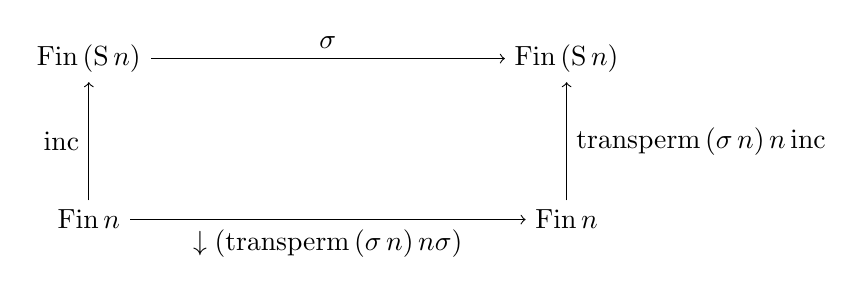
\begin{tikzpicture}[node distance=1.5cm and 4.5cm]
  \node (1) {$\Fin\,(\Suc n)$};
  \node (2) [right=of 1] {$\Fin\,(\Suc n)$}
    edge[<-] node[above] {$\sigma$} (1);
  \node (3) [below=of 1] {$\Fin n$}
    edge[->] node[left] {$\inc$} (1);
  \node (4) [below=of 2] {$\Fin n$}
    edge[<-] node[below] {$\downarrow(\trans\,(\rightarrowtail \sigma\,n)\,n \circ \sigma)$} (3)
    edge[->] node[right] {$\trans\,(\rightarrowtail \sigma\,n)\,n \circ \inc$} (2);
\end{tikzpicture}
\end{center}
which commutes, because taking some arbitrary $m$, if $\rightarrowtail \sigma\,m \equiv n$ then following the diagram we get $n$ both ways, and otherwise the $\trans$s both act as identity and we get $\rightarrowtail \sigma\,m$. We call the construction on the bottom arrow $\sigma^*$.

Next consider the following diagram
\begin{center}
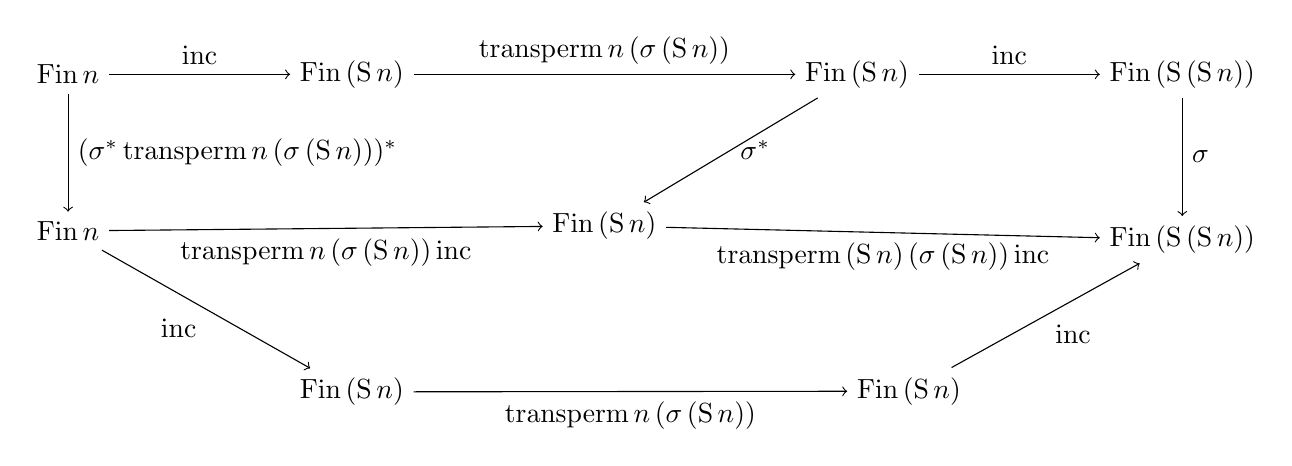
\begin{tikzpicture}[node distance=1.5cm and 2.3cm]
  \node (1) {$\Fin n$};
  \node (2) [right=of 1] {$\Fin\,(\Suc n)$}
    edge[<-] node[above] {$\inc$} (1);
  \node (ghost1) [right=of 2] {};
  \node (3) [right=of ghost1] {$\Fin\,(\Suc n)$}
    edge[<-] node[above] {$\trans n\,(\leftarrowtail \sigma\,(\Suc n))$} (2);
  \node (4) [right=of 3] {$\Fin\,(\Suc\,(\Suc n))$}
    edge[<-] node[above] {$\inc$} (3);
  \node (5) [below=of 1] {$\Fin n$}
    edge[<-] node[right] {$(\sigma^* \circ \trans n\,(\leftarrowtail \sigma\,(\Suc n)))^*$} (1);
  \node (6) [below=of ghost1] {$\Fin\,(\Suc n)$}
    edge[<-] node[below] {$\trans n\,(\rightarrowtail \sigma\,(\Suc n)) \circ \inc$} (5)
    edge[<-] node[right] {$\sigma^*$} (3);
  \node (7) [below=of 4] {$\Fin\,(\Suc\,(\Suc n))$}
    edge[<-] node[below] {$\trans\,(\Suc n)\,(\rightarrowtail \sigma\,(\Suc n)) \circ \inc$} (6)
    edge[<-] node[right] {$\sigma$} (4);
  \node (8) [below right=of 5] {$\Fin\,(\Suc n)$}
    edge[<-] node[below left] {$\inc$} (5);
  \node (9) [below right=of 6] {$\Fin\,(\Suc n)$}
    edge[<-] node[below] {$\trans n\,(\rightarrowtail \sigma\,(\Suc n))$} (8)
    edge[->] node[below right] {$\inc$} (7);
\end{tikzpicture}
\end{center}
The top line and $\sigma$ form the right-hand side of the claim and the bottom three arrow the left-hand side. Therefore the $\Fin n \to \Fin n$ on the left represents the constructed $\sigma'$. The top right quadrangle of this diagram is an instance of the $\sigma^*$ construction above. The top left is another instance, which gives us the $\sigma'$ we need. Finally we need to show that the bottom quadrangle commutes. Take an arbitrary $m$ and assume $m \equiv\,\rightarrowtail \sigma\,(\Suc n)$. Along the top this gives $n$. Along the bottom it also gives $n$. Now assume $m \nequiv \rightarrowtail \sigma\,(\Suc n)$, in which case $m$ is unaffected by all the $\trans$s, so in both cases we get $m$.

\paragraph{Coherence}

Proving that the proof of $\monfold$ is coherent turned out to be extremely difficult, even on paper, so has not been formalised. However, we believe that it should indeed hold, so chose to postulate the result in Agda.

\paragraph{Proofs of Universality} We again need to show that this definition satisfies the necessary conditions to be the free construction as outlined in \Cref{sec:hsetmodel}. The unit law follows by computation as
\begin{align*}
  \monfold f\,\botrec\,(\leftarrowtail \finempty) &\equiv \monfold' 0\,f\,(\botrec \circ {\leftarrowtail \finempty}) \\
  &\equiv e
\end{align*}
The singleton law follows similarly, but requires a call to the right unit law.

The multiplication law is more complex. It has type
$$\Pi_{(x , y : \SM C)}~f^\#\,(x \cup y) = f^\#\,x \otimes f^\#\,y$$
which takes two $\SM C$ values. We would like to perform induction on the size of $x$. The base case is provable because any $\SM C$ of size $0$ is equivalent to $\varnothing$ and then the left unit law applies. However, the inductive case doesn't work out. This is because we cannot split an arbitrary $\SM C$ of size $\Suc n$ to perform induction on the smaller component.

Instead of induction on the size of $x$ we need a new tactic. Intuitively it should be the case that for some property $P$, if $P$ holds for all $\Fin n$ then $P$ should hold for all $I$ equivalent to some $\Fin n$. We want some elimination principle for $\SM C$ that allows us to only consider the case where $I$ is a $\Fin n$. We can construct such a principle using a lemma from \citep{hou2017higher}. First we define surjectivity in homotopy type theory as
$$\mathrm{is\mhyphen surj}\,f \defeq \Pi_{(b : B)}\,\| \Sigma_{(a : A)}\,f\,a = b \|_{-1}.$$
The lemma states that for types $A$ and $B$ and a dependent type $C$ over $B$, for any surjective function $f : A \to B$ and any function $g : \Pi_{(a : A)}\,C\,(f\,a)$ such that
$$\mathrm{g\mhyphen is\mhyphen const} : \Pi_{(a , a' : A)}\Pi_{(p : f\,a = f\,a')}\,g\,a = g\,a'\,[C \downarrow p]$$
there exists a function $h : \Pi_{(b : B)}\,C\,b$ such that $\Pi_{(a : A)}\,h\,(f\,a) = g\,a$.

So consider the function
\begin{align*}
  & \smfin : \Sigma_{(n : \mathbb{N})}\,(\Fin n \to C) \to \SM C \\
  & \smfin\,(n , f) = (\Fin n , f , n , | \mathrm{ide}\,(\Fin n) |)
\end{align*}
This is clearly surjective, which means we can use the lemma above to write an elimination principle. The principle says that to show a function for all $\SM C$ it is enough to show it for all $\smfin\,(n , f)$ and show that it is constant.

Now, for example, to show the multiplication law for the universal property we can use the elimination rule twice, so we need to show
\begin{align*}
  &\Pi_{(m , n : \mathbb{N})}\Pi_{(i : \Fin m \to C)}\Pi_{(j : \Fin n \to C)} \\
  &f^\#\,(\smfin\,(m , i) \cup \smfin\,(n , j)) = f^\#\,(\smfin\,(m , i)) \otimes f^\#\,(\smfin\,(n , j))
\end{align*}
which we can prove by induction because we have concrete values for the truncated equivalences. Then we need to show that this context is constant, which we have not managed to show yet.

\section{Agda Formalisation}

The truncated $\SM$ defines all the concepts from \Cref{subsec:setformal}, therefore the following listings contain only auxiliary concepts used in defining the core ones.

\subsection{Imposed Finiteness}

\begin{center}
\begin{tabular}{ll}
  Concept & Agda Name \\
  \hline
  $\SM$ Truncation level & \texttt{SM-level} \\
  $\finempty$ & \texttt{Fin0-$\bot$} \\
  $\finunit$ & \texttt{Fin1-$\top$} \\
  Coproduct Unit Left & \texttt{$\sqcup$-unit-l} \\
  Coproduct Unit Right & \texttt{$\sqcup$-unit-r} \\
  Coproduct Associativity & \texttt{$\sqcup$-assoc} \\
  Coproduct Comm & \texttt{$\sqcup$-comm} \\
\end{tabular}
\end{center}

\subsection{Functions from Propositional Truncations}

\begin{center}
\begin{tabular}{ll}
  Concept & Agda Name \\
  \hline
  Universal Property for Sets & \texttt{Trunc-to-set-equiv} \\
  Universal Property for Groupoids & \texttt{Trunc-to-gpd-equiv} \\
\end{tabular}
\end{center}

\subsection{The Universal Property}

\begin{center}
\begin{tabular}{ll}
  Concept & Agda Name \\
  \hline
  Transpose Permutation & \texttt{trans-perm} \\
  Transpose Perm Identity & \texttt{trans-perm-id} \\
  Transpose Perm Symmetric & \texttt{trans-perm-sym} \\
  Transpose Perm Applied to Left Value & \texttt{trans-perm-->-l} \\
  Transpose Perm Applied to Right Value & \texttt{trans-perm-->-r} \\
  Transpose Perm Self Inverse & \texttt{trans-perm-double-idf} \\
  $\downarrow$ & \texttt{perm-down} \\
  Inc Composed with $\downarrow$ & \texttt{perm-down-inc} \\
  $\sigma^*$ Construction & \texttt{perm-down-*} \\
  Permutation Invariance of $\monfold'$ & \texttt{monoid-fold'-is-perm-invariant} \\
  Finite $\SM$ Construction & \texttt{SM-Fin} \\
  Finite $\SM$ Construction Surjective & \texttt{SM-Fin-surj} \\
  Splitting Finite $\SM$ Construction & \texttt{SM-Fin-S-split} \\
  $\SM$ Elimination Principle & \texttt{SM-elim} \\
\end{tabular}
\end{center}

This formalisation turned out to require almost identical coherence conditions to the $\hGpd$ model, so again these were postulated. We were also not able to formalise the coherence of $\monfold$, so this was also postulated.

\chapter{Generalised Species of Structures}

Generalised species of structures \citep{fiore2008cartesian} are defined as
$$C \rightwavearrow D \defeq \SM C \to \widehat{D},$$
for types $C$ and $D$. Taking $C$ and $D$ as $\hGpd$s, species are the morphisms of the category $\Esp$. The proofs of the categorical structure are simpler to define in the opposite category $\op\Esp$ so we will begin there.

\section{The Category $\op\Esp$}

The category $\op\Esp$ has objects as $\hGpd$s and homs as functors
$$C \leftwavearrow D \defeq C \to \widehat{\SM D}$$
between $\hGpd$s.

The identity morphism for an $\hGpd$, $C$, is given by
$$\id_C \defeq Y \circ [\_]$$
combining the singleton of $\SM$ and the Yoneda functor.

Composition of morphisms $G : D \leftwavearrow E$ and $F : C \leftwavearrow D$ is defined as
$$G \circ F \defeq \Lan_Y G^\# \circ F.$$
To understand this, consider the following diagram
\begin{center}
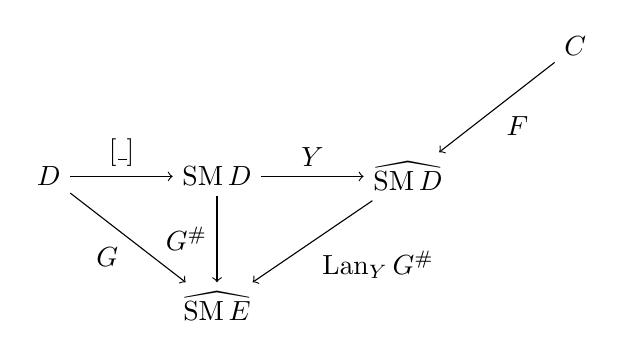
\begin{tikzpicture}[node distance=1.1cm and 1.3cm]
  \node (1) {$D$};
  \node (2) [right=of 1] {$\SM D$}
    edge[<-] node[above] {$[\_]$} (1);
  \node (3) [right=of 2] {$\widehat{\SM D}$}
    edge[<-] node[above] {$Y$} (2);
  \node (4) [above right=of 3] {$C$}
    edge[->] node[below right] {$F$} (3);
  \node (5) [below=of 2] {$\widehat{\SM E}$}
    edge[<-] node[below left] {$G$} (1)
    edge[<-] node[left] {$G^\#$} (2)
    edge[<-] node[below right] {$\Lan_Y G^\#$} (3);
\end{tikzpicture}
\end{center}
The left-hand triangle is an application of the universal property for $\SM$ and the right-hand triangle is an application of the left Kan extension for the Yoneda functor. Composing the resulting morphism with $F$ gives us a morphism of type $C \to \widehat{\SM E}$ as needed.

For the left unit law consider the diagram
\begin{center}
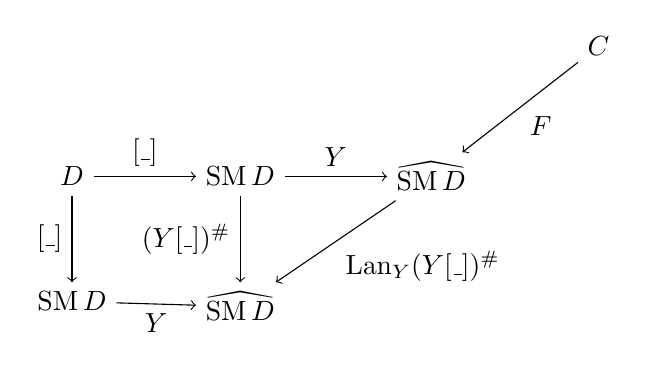
\begin{tikzpicture}[node distance=1.1cm and 1.3cm]
  \node (1) {$D$};
  \node (2) [right=of 1] {$\SM D$}
    edge[<-] node[above] {$[\_]$} (1);
  \node (3) [right=of 2] {$\widehat{\SM D}$}
    edge[<-] node[above] {$Y$} (2);
  \node (4) [above right=of 3] {$C$}
    edge[->] node[below right] {$F$} (3);
  \node (5) [below=of 2] {$\widehat{\SM D}$}
    edge[<-] node[left] {$(Y \circ [\_])^\#$} (2)
    edge[<-] node[below right] {$\Lan_Y (Y \circ [\_])^\#$} (3);
  \node (6) [below=of 1] {$\SM D$}
    edge[<-] node[left] {$[\_]$} (1)
    edge[->] node[below] {$Y$} (5);
\end{tikzpicture}
\end{center}
We have for a monoid homomorphism $h : D \to E$ and a function $f : C \to D$ that
$$(h \circ f)^\# = h \circ f^\#.$$
The Yoneda functor is a homomorphism, as outlined in \Cref{sec:dayconv}. We also have that the universal property applied to the singleton gives the identity function, so therefore
$$(Y \circ [\_])^\# = Y.$$

Finally $\Lan_Y Y = \id$, so $\Lan_Y Y \circ F = F$.

The right unit law and associativity follow from similar diagrams and applications of lemmas about $\Lan$s, defined in \Cref{sec:lans,sec:dayconv}, and the universal property, so we have a category.

% Go a bit more into which lemmas are used so we can reference them properly

% Talk about the Agda translation of one of the left unit proof

We can now derive the category $\Esp$ by taking the dual of $\op\Esp$. We want to show Cartesian closure of the category $\Esp$, but to do this requires an equivalence that we will look at first.

\section{An Important Equivalence}

To show that species form a Cartesian Closed Category we will need the following equivalence
\begin{equation}
  \label{eqn:coprodprod}
  \SM\,(C \sqcup D) \simeq \SM C \times \SM D.
\end{equation}
To show this we need to exhibit a function in each direction and show that both compositions are equal to the identity.

The function in the first direction has type $\SM\,(C \sqcup D) \to \SM C \times \SM D$, so we can use the universal property for $\SM$. Therefore we want to define a function $f : C \sqcup D \to \SM C \times \SM D$. Such a function can be defined as
\begin{align*}
  f (\inl~c) &\defeq ([c] , \varnothing) \\
  f (\inr~d) &\defeq (\varnothing , [d])
\end{align*} and the first direction becomes $f^\#$.

In the opposite direction the function has type $\SM C \times \SM D \to \SM\,(C \sqcup D)$, so we cannot use the universal property directly. Instead, we can apply the functorial action of $\SM$ to the injection functions, to get $$\SM \inl : \SM C \to \SM~(C \sqcup D)$$ and $$\SM \inr : \SM D \to \SM~(C \sqcup D).$$ These can be applied to the left and right components respectively and the results joined with the union operation. The resulting function is
$$g~(c , d) \defeq \SM \inl c \cup \SM \inr d.$$

For the first composition consider the following diagram
\begin{center}
\footnotesize
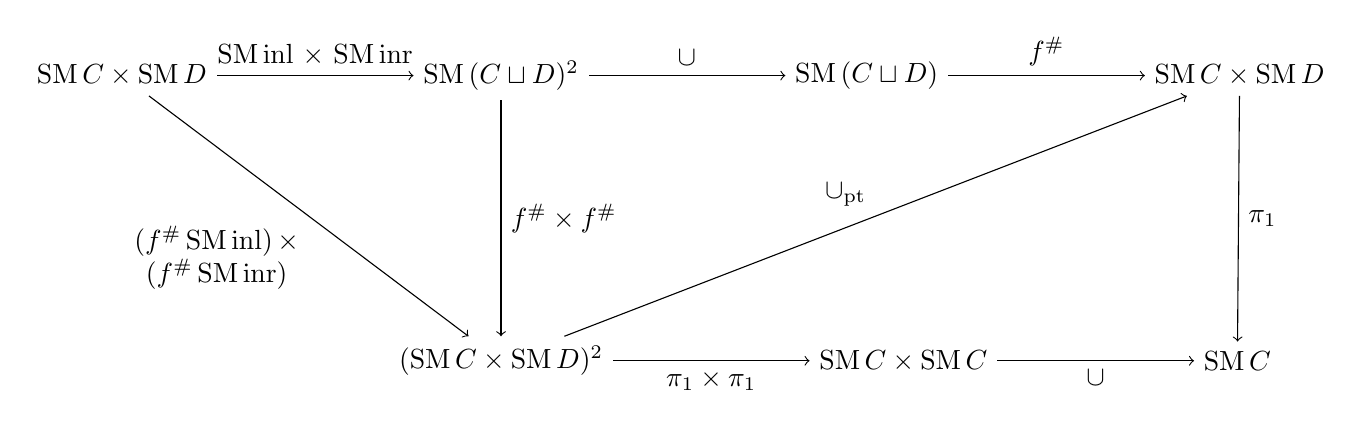
\begin{tikzpicture}[node distance=3cm and 2.5cm,align=center]
\node (1) {$\SM C \times \SM D$};
\node (2) [right=of 1] {$\SM\,(C \sqcup D)^2$}
  edge[<-] node[above] {$\SM \inl$ $\times$ $\SM \inr$} (1);
\node (3) [right=of 2] {$\SM\,(C \sqcup D)$}
  edge[<-] node[above] {$\cup$} (2);
\node (4) [right=of 3] {$\SM C \times \SM D$}
  edge[<-] node[above] {$f^\#$} (3);
\node (5) [below=of 2] {$(\SM C \times \SM D)^2$}
  edge[<-] node[right] {$f^\# \times f^\#$} (2)
  edge[<-] node[below left] {$(f^\# \circ \SM \inl)\,\times$\\ $(f^\# \circ \SM \inr)$} (1)
  edge[->] node[above left] {$\cup_{\mathrm{pt}}$} (4);
\node (6) [right=of 5] {$\SM C \times \SM C$}
  edge[<-] node[below] {$\pi_1 \times \pi_1$} (5);
\node (7) [right=of 6] {$\SM C$}
  edge[<-] node[below] {$\cup$} (6)
  edge[<-] node[right] {$\pi_1$} (4);
\end{tikzpicture}
\end{center}

The top three arrows give the composition in question. We first show that this diagram commutes. Then, if the bottom three arrows give $\pi_1$ and in the same diagram with $\pi_2$s give $\pi_2$, then the whole composition is equal to the identity.

The left-hand triangle commutes by definition. The upper right-hand triangle commutes because the universal extension of $f$ is a monoid homomorphism. $\cup$ is the associative operation of the monoid on $\SM$. $\cup_{\mathrm{pt}}$ applies this operation pointwise, which is the extension of the monoid structure to a pair of monoids. The lower right-hand triangle commutes because $\pi_1$ is a monoid homomorphism.

To show that the bottom three arrows give $\pi_1$ we need a couple of things. Firstly consider the following diagram
\begin{center}
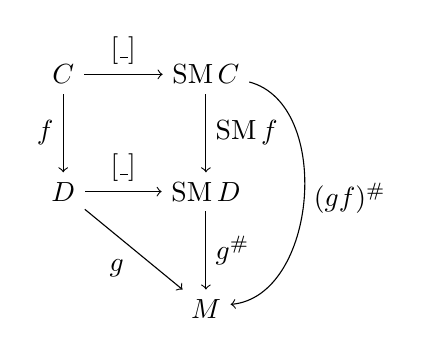
\begin{tikzpicture}
\node (1) {$C$};
\node (2) [right=of 1] {$\SM C$}
  edge[<-] node[above] {$[\_]$} (1);
\node (3) [below=of 1] {$D$}
  edge[<-] node[left] {$f$} (1);
\node (4) [below=of 2] {$\SM D$}
  edge[<-] node[above] {$[\_]$} (3)
  edge[<-] node[right] {$\SM f$} (2);
\node (5) [below=of 4] {$M$}
  edge[<-] node[below left] {$g$} (3)
  edge[<-] node[right] {$g^\#$} (4)
  edge[<-,bend right=80] node[right] {$(g \circ f)^\#$} (2);
\end{tikzpicture}
\end{center}
Clearly the composition of two monoid homomorphism is a monoid homomorphism. We can therefore use the uniqueness of the universal property to get
$$g^\# \circ \SM f = (g \circ f)^\#.$$ Secondly for two functions $f : C \to D$ and $g : C \to E$ we have
$$\langle f , g \rangle^\# = \langle f^\# , g^\# \rangle,$$
again as a consequence of uniqueness.

Using these, for a pair $(c , d) : \SM C \times \SM D$ we get
\begin{align*}
  &\quad\  \pi_1 (f^\# (\SM \inl c)) \cup \pi_1 (f^\# (\SM \inr d)) \\
  &= \pi_1 ((f \circ \inl)^\#~c) \cup \pi_1 ((f \circ \inr)^\#~d) &&\text{(first property above)} \\
  &\equiv \pi_1 ((\lambda~c \to ([c] , \varnothing))^\#~c) \cup \pi_1 ((\lambda~d \to (\varnothing , [d]))^\#~d) \\
  &= \pi_1 (\langle [\_]^\# , (\mathrm{cst}~\varnothing)^\# \rangle~c) \cup \pi_1 (\langle (\mathrm{cst}~\varnothing)^\# , [\_]^\# \rangle~d) &&\text{(second property above)}\\
  &= \pi_1 (c , \varnothing) \cup \pi_1 (\varnothing , d) &&\text{(universal property for $[\_]$ and $\mathrm{cst}~\varnothing$)}\\
  &\equiv c \cup \varnothing \\
  &= c &&\text{(right unit law)} \\
  &\equiv \pi_1 (c , d)
\end{align*}
as required, and get a similar result for $\pi_2$.

For the second composition we show that $g \circ f^\#$ is a monoid homomorphism and that
$$g~(f~[c]) = [c].$$
This implies that $g \circ f = [\_]^\#$ by uniqueness of the universal property.
We have that $[\_]^\# = \mathrm{id}$, so $g \circ f = id$.

% Maybe include agda code for one direction and compare

\section{Cartesian Closure of $\Esp$}

The terminal object of $\Esp$ is an $\hGpd$, $\top_1$, such that for any other $\hGpd$, $C$, there is a unique morphism $C \rightwavearrow \top_1$. A morphism $C \rightwavearrow \top_1$ is a function
$$\top_1 \to \SM C \to \mathcal{U}$$
so we need a $\top_1$ such that the function space $\top_1 \to D$ is contractible for all $D$. This is satisfied by $\bot$, for which $\botrec$ is the unique function from $\bot$ to any other type.

The product of two $\hGpd$s in $\Esp$ is given by the coproduct, $\sqcup$. That this is a categorical product is proved using the equivalence
$$C \rightwavearrow D \sqcup E \simeq (C \rightwavearrow D) \times (C \rightwavearrow E)$$ which is simple to define. The forward direction is defined by
$$f\,h \defeq ((\lambda\,d\,c \to h\,(\inl d)\,c) , (\lambda\,e\,c \to h\,(\inr e)\,c))$$
and the backward direction by
\begin{align*}
  g\,(h_1 , h_2)\,(\inl d) &\defeq h_1\,d \\
  g\,(h_1 , h_2)\,(\inr e) &\defeq h_2\,e
\end{align*}
and these can easily be seen to be inverses.

The exponential object $C \Rightarrow D$ is defined as
$$C \Rightarrow D \defeq \SM C \times D.$$ That this is indeed an exponential is proved using the equivalence
$$C \sqcup D \rightwavearrow E \simeq C \rightwavearrow D \Rightarrow E.$$
We have
\begin{align*}
  C \sqcup D \rightwavearrow E &\equiv E \to \reallywidehat{\SM\,(C \sqcup D)} \\
  &\simeq E \to \reallywidehat{\SM C \times \SM D} &&\text{(\Cref{eqn:coprodprod})} \\
  &\simeq \SM D \times E \to \widehat{\SM C} &&\text{(Currying, reordering, uncurrying)} \\
  &\equiv C \rightwavearrow D \Rightarrow E
\end{align*}

\section{The Differential Calculus of Species}

We now define the differential calculus of species \citep{fiore2005mathematical}, a set of operations on species that obey rules analogous to those of analysis.

\paragraph{Addition} The $\boxplus$ operation behaves like addition. It is a binary operation that takes two species of the same type and returns a third. For two presheaves $P , Q : \spec{C}{D}$, the definition is
$$(P \boxplus Q)\,d\,m \defeq (P\,d\,m) \sqcup (Q\,d\,m).$$
The unit for this operation is
$$0\,d\,m \defeq \bot$$
which satisfies left and right unit laws. They hold because we have
$$\bot \sqcup C \simeq C$$
and
$$C \sqcup \bot \simeq C$$
which we used when defining the union of the truncated version of $\SM$. This operation is also commutative and associative, again from the commutativity and associativity of $\sqcup$. This also distributes with species composition as
$$\Pi_{(P : \spec{C}{D})}\Pi_{(Q , R : \spec{D}{E})}\,(Q \boxplus R) \circ P = (Q \circ P) \boxplus (R \circ P),$$
which follows from the action of $\Lan_Y$ on $\sqcup$, defined in \Cref{sec:lans}.

\paragraph{Multiplication} The $\boxtimes$ operation behaves like multiplication. For two species $P , Q : \spec{C}{D}$, the definition is
$$(P \boxtimes Q)\,d \defeq (P\,d \daytensor Q\,d).$$
The unit for this operation is
$$1\,d \defeq \hat{I},$$
which satisfies the unit laws because of the unit laws for $\daytensor$. This operation is commutative and associative, again from $\daytensor$. It also distributes with species composition as
$$\Pi_{(P : \spec{C}{D})}\Pi_{(Q , R : \spec{D}{E})}\,(Q \boxtimes R) \circ P = (Q \circ P) \boxtimes (R \circ P),$$ which follows from $\Lan_Y P^\#$ being a monoid homomorphism, as defined in \Cref{sec:dayconv}.

% Further we have distributivity laws, defined by...

\paragraph{Differentiation} The $\partial$ operation behaves as a partial derivative. Given an $c : C$ and a species $P : \spec{C}{D}$ it gives a new $\spec{C}{D}$. The definition is
$$\partial\,c\,P\,d\,m \defeq P\,d\,(m \cup [c]).$$

For intuition about this operation, take $C$ and $D$ to be $\top$. Now $$\spec{\top}{\top} \equiv \top \to \widehat{\SM \top} \simeq \widehat{\SM \top}.$$ $\SM \top$ corresponds to the groupoid of finite sets and bijections, $\mathbb{B}$, so $\widehat{\SM \top}$ corresponds to the species of \citet{joyal1981une}. For $P : \widehat{\SM \top}$ we get a functorial action on morphisms and uncurrying this we get
$$P_n \times \widehat{\SM \top}(n,n) \to P_n,$$
which can be seen as a quotient of $P_n$ by permutations. There are $n!$ such permutations, so we can use these as the coefficients of an exponential power series
$$p(x) = \sum_{n \geq 0}~P_n~\frac{x^n}{n!}$$
which differentiates to
$$p'(x) = \sum_{n \geq 0}~P_n~\frac{x^{n-1}}{(n-1)!}.$$ We can see this as
$$p'(x) = \sum_{i \geq 0}~P_{i+1}~\frac{x^i}{i!},$$ so differentiation shifts the index by 1. So now for an arbitrary $C$, we can shift in any direction $c$ by adding 1 value of this element to the multiset.

This operation satisfies some commutativity property
$$\Pi_{(c , c' : C)}\,\partial\,c\,(\partial\,c'\,P) = \partial\,c'\,(\partial\,c\,P),$$ which holds by associativity and commutativity of $\cup$. It also satisfies
$$\Pi_{(c : C)}\Pi_{(P , Q : \spec{C}{D})}\,\partial\,c\,(P \boxplus Q) = \partial\,c\,P \boxplus \partial\,c\,Q,$$
and
$$\Pi_{(c : C)}\,\partial\,c\,E = E,$$ where $E$ is the constantly $\top$ presheaf of two arguments, named for its analogy to Euler's number, $e$. Both of these hold judgmentally.

We can also define the operation $\delta$, which given a species $\spec{C}{D}$ returns a species $\spec{C}{C \times D}$ and is defined by
$$\delta\,P\,(c , d)\,m \defeq \partial\,c\,P\,d\,m.$$
This corresponds to the Jacobian matrix which for some $f : \mathbb{R}^n \to \mathbb{R}^m$ is an $m \times n$ matrix of partial derivatives. Given some $j : \mathbb{R}^n$ we get a linear operator from $\mathbb{R}^n$ to $\mathbb{R}^m$ by taking the appropriate column of the matrix. This map
$$\mathbb{R}^n \to \mathrm{Lin}(\mathbb{R}^n,\mathbb{R}^m)$$
corresponds to our
$$\spec{C}{C \times D}.$$

With these operations we can prove the Leibniz Rule
$$\partial_c\,(P \cdot Q) = \partial_c(P) \cdot Q + P \cdot \partial_c(Q)$$
which translates to
$$\partial\,c\,(P \boxtimes Q) = (\partial\,c\,P \boxtimes Q) \boxplus (P \boxtimes \partial\,c\,Q).$$
We have
\begin{align*}
  &\quad\ \partial\,c\,(P \boxtimes Q)\,d\,m \\
  &\equiv (P \boxtimes Q)\,d\,(m \cup [c]) \\
  &\equiv \Sigma_{(m_1 , m_2 : \SM C)}\,P\,d\,m_1 \times Q\,d\,m_2 \times (m \cup [c] = m_1 \cup m_2) \\
  &= \Sigma_{(m_1 , m_2 : \SM C)}\,P\,d\,m_1 \times Q\,d\,m_2 \\
  &\qquad\qquad\qquad\times ((\Sigma_{(m' : \SM C)}\,(m = m' \cup m_2) \times (m' \cup [c] = m_1)) \\
  &\qquad\qquad\qquad\quad\sqcup \\
  &\qquad\qquad\qquad\quad(\Sigma_{(m' : \SM C)}\,(m = m_1 \cup m') \times (m' \cup [c] = m_2))) &&\text{(combinatorial lemma)}\\
  &=(\Sigma_{(m_1 , m_2 : \SM C)}\,P\,d\,m_1 \times Q\,d\,m_2  \\
  &\qquad\qquad\qquad\,\times \Sigma_{(m' : \SM C)}\,(m = m' \cup m_2) \times (m' \cup [c] = m_1)) \\
  &\quad\ \sqcup \\
  &\quad\ (\Sigma_{(m_1 , m_2 : \SM C)}\,P\,d\,m_1 \times Q\,d\,m_2  \\
  &\qquad\qquad\qquad\,\times \Sigma_{(m' : \SM C)}\,(m = m_1 \cup m') \times (m' \cup [c] = m_2)) \\
  &=(\Sigma_{(m' , m_2 : \SM C)}\,P\,d\,(m' \cup [c]) \times Q\,d\,m_2 \times (m = m' \cup m_2)) \\
  &\quad\ \sqcup \\
  &\quad\ (\Sigma_{(m_1 , m' : \SM C)}\,P\,d\,m_1 \times Q\,d\,(m' \cup [c]) \times (m = m_1 \cup m')) &&\text{(density formula twice)} \\
  &\equiv (\partial\,c\,P \boxtimes Q) \boxplus (P \boxtimes \partial\,c\,Q)
\end{align*}
The most difficult step in this proof is the \emph{combinatorial lemma} which has type
\begin{align*}
  &(m \cup [c] = m_1 \cup m_2) \\
  &\simeq \\
  &((\Sigma_{(m' : \SM C)}\,(m = m' \cup m_2) \times (m' \cup [c] = m_1)) \sqcup (\Sigma_{(m' : \SM C)}\,(m = m_1 \cup m') \times (m' \cup [c] = m_2)))
\end{align*}
This was left as a postulate, because the proof too complicated for the amount of time, but intuitively we should be able to split up $m$ based on $c$'s membership in $m_1$ or $m_2$.

\section{Agda Formalisation}

\subsection{The Category $\op\Esp$}

\begin{center}
\begin{tabular}{ll}
  Concept & Agda Name \\
  \hline
  $\leftwavearrow$ & $\_\leftwavearrow\_$ \\
  Identities & \texttt{id$_2$} \\
  Composition & $\_\circ_2\_$ \\
  Composition Unit Left & \texttt{$\_\circ_2\_$-unit-l} \\
  Composition Unit Right & \texttt{$\_\circ_2\_$-unit-r} \\
  Composition Associativity & \texttt{$\_\circ_2\_$-assoc} \\
  Composition Commutativity & \texttt{$\_\circ_2\_$-comm} \\
  Universal Extension of Composition & \texttt{lan-y-$\circ$-up} \\
\end{tabular}
\end{center}

\subsection{An Important Equivalence}

\begin{center}
\begin{tabular}{ll}
  Concept & Agda Name \\
  \hline
  $\pi_1$ Homomorphism Mult & \texttt{fst-hom-mult} \\
  $\pi_2$ Homomorphism Mult & \texttt{snd-hom-mult} \\
  Universal Extension on Pairs & \texttt{up-pair} \\
  $\SM$ Functor Composed with Universal Property & \texttt{SM-fmap-up} \\
  $\SM$ Coproduct/Product Equivalence & \texttt{SM-$\sqcup$-$\times$-equiv} \\
\end{tabular}
\end{center}

\subsection{Cartesian Closure of $\Esp$}

\begin{center}
\begin{tabular}{ll}
  Concept & Agda Name \\
  \hline
  Product in $\Esp$ & $\_\times_\texttt{s}\_$ \\
  Product Equivalence & \texttt{$\times_\texttt{s}$-equiv} \\
  Exponential in $\Esp$ & $\_\Rightarrow_\texttt{s}\_$ \\
  Exponential Equivalence & \texttt{$\Rightarrow_\texttt{s}$-equiv} \\
\end{tabular}
\end{center}

\subsection{The Differential Calculus of Species}

\begin{center}
\begin{tabular}{ll}
  Concept & Agda Name \\
  \hline
  Addition & $\_\boxplus\_$ \\
  $0$ & $0_\texttt{s}$ \\
  Addition Unit Left & \texttt{$\boxplus$-unit-l} \\
  Addition Unit Right & \texttt{$\boxplus$-unit-r} \\
  Addition Unit Associativity & \texttt{$\boxplus$-assoc} \\
  Addition Unit Commutativity & \texttt{$\boxplus$-comm} \\
  Addition Distributivity over Composition & \texttt{$\boxplus$-$\circ_\texttt{s}$-l} \\
  Multiplication & $\_\boxtimes\_$ \\
  $1$ & $1_\texttt{s}$ \\
  Multiplication Unit Left & \texttt{$\boxtimes$-unit-l} \\
  Multiplication Unit Right & \texttt{$\boxtimes$-unit-r} \\
  Multiplication Unit Associativity & \texttt{$\boxtimes$-assoc} \\
  Multiplication Unit Commutativity & \texttt{$\boxtimes$-comm} \\
  Multiplication Distributivity over Composition & \texttt{$\boxtimes$-$\circ_\texttt{s}$-l} \\
  Partial Differentiation & $\partial$ \\
  Partial Diff Commutativity & \texttt{$\partial$-comm} \\
  Partial Diff of Addition & \texttt{$\partial$-$\boxplus$} \\
  Partial Diff of $E$ & \texttt{$\partial$-E} \\
  Leibniz Rule & \texttt{leibniz} \\
  Jacobian & $\delta$ \\
\end{tabular}
\end{center}

\chapter{Summary \& Conclusions}

Overall the project was a success. We were able to define the differential calculus of generalised species of structures for groupoids, which was initially a stretch goal. Both formalisations of the $\SM$ construction led us to the edge of current research. The first required higher-dimensional HITs, the implementation of which was made simpler by the addition of rewrite rules to Agda during the development of this project. The second required stronger universal properties for working with truncated types.

The deliverable of the project, the Agda code itself, represents a significant contribution in terms of formalising this internalised theory of groupoids. It is a foundation on top of which other categorical theories and constructions could be built. At the time of writing we were not able to formalise a number of coherence conditions required by the $\SM$ construction, but we would like to continue working at these even after this project is over.

As mentioned in \Cref{chap:intro} this project represents another test of the worth of Agda and homotopy type theory in aiding formalisation. In general it was a pleasure to work with both of the tools. Programming with holes in Agda quickly became very natural. Homotopy type theory also started to feel very natural, especially coming from a computer science background. The main drawback of Agda was the manipulation of universes, which could be tedious at times.

An interesting question that this project raises, and which has been explored by \citet{kraus2014general}, is that of formalising the theory with arbitrary truncation levels. It is certainly the case that the \emph{definition} of the $\SM$ construction from the truncated formalisation can be used for any (finite) truncation level, but writing the proofs at each subsequent level requires another set of coherence conditions. Whether these coherence conditions, and more importantly proofs of them, can be defined in some level independent way remains an open question. It is conjectured that it is not possible to define the coherence conditions up to infinity within the type theory.

\newpage

\bibliography{dissertation}

\end{document}
